% Chapter 10: Comprehensive Review
% Harvard-quality academic presentation
% Bachelor program, Bucharest University of Economic Studies

\documentclass[9pt, aspectratio=169, t]{beamer}

% Ensure content fits on slides
\setbeamersize{text margin left=8mm, text margin right=8mm}

%=============================================================================
% THEME AND STYLE CONFIGURATION
%=============================================================================
\usetheme{default}
% Using default theme for clean header/footer control

% Color Palette (matching Redispatch PDF)
\definecolor{MainBlue}{RGB}{26, 58, 110}
\definecolor{AccentBlue}{RGB}{26, 58, 110}
\definecolor{IDAred}{RGB}{205, 0, 0}
\definecolor{DarkGray}{RGB}{51, 51, 51}
\definecolor{MediumGray}{RGB}{128, 128, 128}
\definecolor{LightGray}{RGB}{248, 248, 248}
\definecolor{VeryLightGray}{RGB}{235, 235, 235}
\definecolor{KeynoteGray}{RGB}{218, 218, 218}
\definecolor{SectionGray}{RGB}{120, 120, 120}
\definecolor{FooterGray}{RGB}{100, 100, 100}
\definecolor{Crimson}{RGB}{220, 53, 69}
\definecolor{Forest}{RGB}{46, 125, 50}
\definecolor{Amber}{RGB}{181, 133, 63}
\definecolor{Orange}{RGB}{230, 126, 34}
\definecolor{Purple}{RGB}{142, 68, 173}

% Gradient background (exact Keynote 315° gradient: white to RGB 218,218,218)
\setbeamertemplate{background}{%
    \begin{tikzpicture}[remember picture, overlay]
        \shade[shading=axis, shading angle=315,
        top color=white, bottom color=KeynoteGray]
        (current page.south west) rectangle (current page.north east);
    \end{tikzpicture}%
}
% Fallback solid color for compatibility
\setbeamercolor{background canvas}{bg=}

\setbeamercolor{palette primary}{bg=MainBlue, fg=white}
\setbeamercolor{palette secondary}{bg=MainBlue!85, fg=white}
\setbeamercolor{palette tertiary}{bg=MainBlue!70, fg=white}
\setbeamercolor{structure}{fg=MainBlue}
\setbeamercolor{title}{fg=IDAred}
\setbeamercolor{frametitle}{fg=IDAred, bg=}
\setbeamercolor{block title}{bg=MainBlue, fg=white}
\setbeamercolor{block body}{bg=VeryLightGray, fg=DarkGray}
\setbeamercolor{block title alerted}{bg=Crimson, fg=white}
\setbeamercolor{block body alerted}{bg=Crimson!8, fg=DarkGray}
\setbeamercolor{block title example}{bg=Forest, fg=white}
\setbeamercolor{block body example}{bg=Forest!8, fg=DarkGray}
\setbeamercolor{item}{fg=MainBlue}

% Footer colors (override Madrid theme blue)
\setbeamercolor{author in head/foot}{fg=FooterGray, bg=}
\setbeamercolor{title in head/foot}{fg=FooterGray, bg=}
\setbeamercolor{date in head/foot}{fg=FooterGray, bg=}
\setbeamercolor{section in head/foot}{fg=FooterGray, bg=}
\setbeamercolor{subsection in head/foot}{fg=FooterGray, bg=}

% Bullet styles (apply everywhere including blocks)
\setbeamertemplate{itemize item}{\color{MainBlue}$\boxdot$}
\setbeamertemplate{itemize subitem}{\color{MainBlue}$\blacktriangleright$}
\setbeamertemplate{itemize subsubitem}{\color{MainBlue}\tiny$\bullet$}
\setbeamertemplate{itemize/enumerate body begin}{\normalsize}
\setbeamertemplate{itemize/enumerate subbody begin}{\normalsize}

% Item spacing - compact style
\setlength{\leftmargini}{10pt}       % Level 1: minimal indent
\setlength{\leftmarginii}{10pt}      % Level 2: minimal additional indent
% Compact list spacing (zero extra space before/after lists in blocks)
\makeatletter
\def\@listi{\leftmargin\leftmargini \topsep 0pt \parsep 0pt \itemsep 0pt}
\def\@listii{\leftmargin\leftmarginii \topsep 0pt \parsep 0pt \itemsep 0pt}
\makeatother

\setbeamertemplate{navigation symbols}{}

%=============================================================================
% CUSTOM HEADLINE
%=============================================================================
\setbeamertemplate{headline}{%
    \vskip10pt%
    \hbox to \paperwidth{%
        \hskip0.5cm%
        {\small\color{FooterGray}\renewcommand{\hyperlink}[2]{##2}\insertsectionhead}%
        \hfill%
        \textcolor{FooterGray}{\small\insertframenumber}%
        \hskip0.5cm%
    }%
    \vskip4pt%
    {\color{FooterGray}\hrule height 0.4pt}%
}

%=============================================================================
% CUSTOM FOOTER
%=============================================================================
\usepackage{fontawesome5}

\setbeamertemplate{footline}{%
    {\color{FooterGray}\hrule height 0.4pt}%
    \vskip4pt%
    \hbox to \paperwidth{%
        \hskip0.5cm%
        \textcolor{FooterGray}{\small Time Series Analysis and Forecasting}%
        \hfill%
        \raisebox{-0.1em}{%
            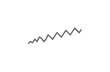
\begin{tikzpicture}[x=0.08em, y=0.08em, line width=0.4pt]
                \draw[FooterGray] (0,3) -- (1,4) -- (2,3.5) -- (3,5) -- (4,4) -- (5,6) -- (6,5.5) -- (7,4) -- (8,5) -- (9,7) -- (10,6) -- (11,5) -- (12,6.5) -- (13,8) -- (14,7) -- (15,6) -- (16,7.5) -- (17,9) -- (18,8) -- (19,7) -- (20,8.5) -- (21,10) -- (22,9) -- (23,8) -- (24,9.5);
            \end{tikzpicture}%
        }%
        \hskip0.5cm%
    }%
    \vskip6pt%
}

%=============================================================================
% PACKAGES
%=============================================================================
\usepackage[utf8]{inputenc}
\usepackage[T1]{fontenc}
\usepackage{amsmath, amssymb, amsthm}
\usepackage{mathtools}
\usepackage{bm}
\usepackage{tikz}
\usetikzlibrary{arrows.meta, positioning, shapes, calc, decorations.pathreplacing, shadings}
\usepackage{booktabs}
\usepackage{multirow}
\usepackage{array}
\usepackage{graphicx}
\usepackage{hyperref}
\usepackage{colortbl}
\hypersetup{colorlinks=true, linkcolor=MainBlue, urlcolor=MainBlue}
\graphicspath{{../../logos/}{../../charts/}}
\hfuzz=2pt  % Suppress tiny overfull warnings (<2pt)
\vfuzz=2pt  % Suppress tiny vertical overfull warnings (<2pt)

%=============================================================================
% QUANTLET COMMAND
%=============================================================================
\newcommand{\quantlet}[2]{%
    \hfill\href{#2}{%
        \raisebox{-0.15em}{\includegraphics[height=0.7em]{ql_logo.png}}%
        \textcolor{MainBlue}{\tiny\ #1}%
    }%
}

%=============================================================================
% CUSTOM TITLE PAGE
%=============================================================================
\defbeamertemplate*{title page}{hybrid}[1][]
{
    \vspace{0.2cm}
    % Logos row - top header (with clickable links)
    \begin{center}
        \href{https://www.ase.ro}{\includegraphics[height=1.0cm]{ase_logo.png}}\hspace{0.3cm}%
        \href{https://theida.net}{\includegraphics[height=1.0cm]{ida_logo.png}}\hspace{0.3cm}%
        \href{https://blockchain-research-center.com}{\includegraphics[height=1.0cm]{brc_logo.png}}\hspace{0.3cm}%
        \href{https://www.ai4efin.ase.ro}{\includegraphics[height=1.0cm]{ai4efin_logo.png}}\hspace{0.3cm}%
        \href{https://ipe.ro/new}{\includegraphics[height=1.0cm]{acad_logo.png}}\hspace{0.3cm}%
        \href{https://www.digital-finance-msca.com}{\includegraphics[height=1.0cm]{msca_logo.png}}%
    \end{center}

    \vspace{0.6cm}

    % Main title with Q logos on sides (with clickable links)
    \begin{center}
        \begin{minipage}{0.1\textwidth}
            \centering
            \href{https://quantlet.com}{\includegraphics[height=1.1cm]{ql_logo.png}}
        \end{minipage}%
        \begin{minipage}{0.78\textwidth}
            \centering
            {\LARGE\bfseries\usebeamercolor[fg]{title}\inserttitle}

            \vspace{0.3cm}

            {\usebeamerfont{subtitle}\usebeamercolor[fg]{title}\insertsubtitle}
        \end{minipage}%
        \begin{minipage}{0.1\textwidth}
            \centering
            \href{https://quantinar.com}{\includegraphics[height=1.1cm]{qr_logo.png}}
        \end{minipage}
    \end{center}

    \vspace{0.6cm}

    % Authors (left aligned)
    \hspace{0.5cm}{\usebeamerfont{author}\insertauthor}

    \vspace{0.3cm}

    % Institute/Affiliations (left aligned)
    \hspace{0.5cm}\begin{minipage}[t]{0.9\textwidth}
        \raggedright\small\insertinstitute
    \end{minipage}
}

%=============================================================================
% THEOREM ENVIRONMENTS
%=============================================================================
\theoremstyle{definition}
\setbeamertemplate{theorems}[numbered]
\newtheorem{defn}{Definition}
\newtheorem{thm}{Theorem}
\newtheorem{prop}{Proposition}
\newtheorem{rmk}{Remark}

%=============================================================================
% CUSTOM COMMANDS
%=============================================================================
\newcommand{\E}{\mathbb{E}}
\newcommand{\Var}{\text{Var}}
\newcommand{\Cov}{\text{Cov}}
\newcommand{\Corr}{\text{Corr}}
\newcommand{\R}{\mathbb{R}}
\newcommand{\N}{\mathbb{N}}
\newcommand{\Z}{\mathbb{Z}}
\newcommand{\B}{\mathbf{B}}
\newcommand{\imark}{\textcolor{MainBlue}{\textbullet}}
\newcommand{\RMSE}{\text{RMSE}}
\newcommand{\MAE}{\text{MAE}}
\newcommand{\MAPE}{\text{MAPE}}

%=============================================================================
% TITLE INFORMATION
%=============================================================================
\title[Time Series Analysis]{Time Series Analysis and Forecasting}
\subtitle{Chapter 10: Comprehensive Review}
\author[D.T. Pele]{Daniel Traian PELE}
\institute{Bucharest University of Economic Studies\\
IDA Institute Digital Assets\\
Blockchain Research Center\\
AI4EFin Artificial Intelligence for Energy Finance\\
Romanian Academy, Institute for Economic Forecasting\\
MSCA Digital Finance}
\date{}

%=============================================================================
% CENTRED MINIPAGE
%=============================================================================
\newenvironment{cminipage}[1]{%
    \par\noindent\hfill\begin{minipage}{#1}\ignorespaces
}{%
    \end{minipage}\hfill\null\par
}

\begin{document}

% Title page (no header/footer)
{
\setbeamertemplate{headline}{}
\setbeamertemplate{footline}{}
\begin{frame}
    \titlepage
\end{frame}
}

%=============================================================================
% LEARNING OBJECTIVES
%=============================================================================
\begin{frame}{Learning Objectives}
    \begin{cminipage}{0.95\textwidth}
\begin{block}{By the end of this chapter, you will be able to:}
\begin{itemize}\setlength{\itemsep}{0pt}
    \item Apply the complete forecasting workflow from data to evaluation
    \item Select appropriate models based on data characteristics
    \item Evaluate forecast accuracy using proper metrics and cross-validation
    \item Integrate knowledge from all previous chapters in practice
\end{itemize}
\end{block}
    \end{cminipage}
\end{frame}

%=============================================================================
% TABLE OF CONTENTS
%=============================================================================
\begin{frame}{Outline}
    \vspace{-0.3cm}
    {\small
    \tableofcontents
    }
\end{frame}

%=============================================================================
% SECTION 1: METHODOLOGY
%=============================================================================
\section{Forecasting Methodology}

\begin{frame}{The Scientific Approach to Forecasting}
    \begin{cminipage}{0.95\textwidth}
    \begin{block}{Research Question}
        How do we \textbf{rigorously evaluate} forecast performance while avoiding overfitting?
    \end{block}

    \vspace{0.3cm}

    \begin{alertblock}{The Fundamental Problem}
        \begin{itemize}\setlength{\itemsep}{0pt}
            \item In-sample fit $\neq$ Out-of-sample performance
            \item Models can ``memorize'' training data without learning patterns
            \item \textbf{Solution}:
                \begin{itemize}\setlength{\itemsep}{0pt}
                    \item Proper train/validation/test methodology
                \end{itemize}
            \end{itemize}
    \end{alertblock}

    \vspace{0.3cm}

    \begin{exampleblock}{Key Principle}
        ``The test set must remain \textbf{untouched} until final evaluation.'' \\
        \hfill --- Standard practice in machine learning and econometrics
    \end{exampleblock}
    \end{cminipage}
\end{frame}

\begin{frame}{Train/Validation/Test Framework}
    \begin{center}
        \includegraphics[width=0.95\textwidth, height=0.78\textheight, keepaspectratio]{../charts/train_val_test_split.pdf}
    \end{center}
    \quantlet{TSA\_ch10\_train\_val\_test\_split}{https://github.com/QuantLet/TSA/tree/main/TSA_ch10/TSA_ch10_train_val_test_split}
\end{frame}

\begin{frame}{Evaluation Metrics}
    \begin{defn}[Forecast Error Metrics]
        Let $y_t$ be actual, $\hat{y}_t$ forecast:
        \vspace{-0.2cm}
        \begin{align*}
            \RMSE = \sqrt{\frac{1}{n}\sum_{t}(y_t - \hat{y}_t)^2}, \quad
            \MAE = \frac{1}{n}\sum_{t}|y_t - \hat{y}_t|, \quad
            \MAPE = \frac{100\%}{n}\sum_{t}\left|\frac{y_t - \hat{y}_t}{y_t}\right|
        \end{align*}
    \end{defn}

    \begin{columns}[T]
        \column{0.5\textwidth}
        \begin{exampleblock}{When to Use Each}
            \begin{itemize}\setlength{\itemsep}{0pt}
                \item \textbf{RMSE}: Penalizes large errors
                \item \textbf{MAE}: Robust to outliers
                \item \textbf{MAPE}: Scale-independent (\%)
            \end{itemize}
        \end{exampleblock}

        \column{0.5\textwidth}
        \begin{alertblock}{Caution}
            \begin{itemize}\setlength{\itemsep}{0pt}
                \item MAPE undefined when $y_t = 0$
                \item Compare on \textbf{same} test set
                \item Report \textbf{out-of-sample} metrics
            \end{itemize}
        \end{alertblock}
    \end{columns}
\end{frame}

\begin{frame}{Forecast Evaluation Beyond RMSE}
    {\small
    \begin{block}{Alternative metrics}
        \begin{itemize}\setlength{\itemsep}{4pt}
            \item \textbf{MASE} (Mean Absolute Scaled Error): $\dfrac{\text{MAE}_{\text{model}}}{\text{MAE}_{\text{naïve}}}$\,; \; $<1 \Rightarrow$ beats naïve
            \item \textbf{DA} (Directional Accuracy): $\dfrac{1}{h}\sum_{t=1}^{h} \mathbf{1}\!\bigl(\text{sgn}\,\Delta\hat{y}_t = \text{sgn}\,\Delta y_t\bigr)$
            \item \textbf{QL} (Quantile Loss): asymmetric penalty $\alpha$ vs $1\!-\!\alpha$
            \[
            QL_{\alpha} =
            \begin{cases}
            \alpha (y_t - \hat{q}_t), & y_t > \hat{q}_t \\
            (1-\alpha)(\hat{q}_t - y_t), & y_t \le \hat{q}_t
            \end{cases}
            \]
            \item \textbf{CRPS} (Continuous Ranked Probability Score): $\displaystyle\int_{-\infty}^{\infty}\!\bigl(F(x) - \mathbf{1}_{x \ge y}\bigr)^{2}dx$
        \end{itemize}
    \end{block}
    }
\end{frame}

\begin{frame}{Forecast Evaluation: Bitcoin Results}
    \begin{columns}[T]
        \column{0.48\textwidth}
        \begin{alertblock}{Bitcoin Results (GARCH volatility)}
            \begin{tabular}{lc}
                \textbf{Metric} & \textbf{Value} \\
                \midrule
                RMSE & 2.21 \\
                MAE & 1.89 \\
                MASE & 0.98 \\
                Dir. Accuracy & 28.7\% \\
            \end{tabular}
            \vspace{0.2cm}
            \begin{itemize}\setlength{\itemsep}{2pt}
                \item MASE $< 1$: GARCH beats naïve
                \item DA 28.7\%: volatility direction is hard
            \end{itemize}
        \end{alertblock}

        \column{0.50\textwidth}
        \begin{block}{Interpretation}
            \begin{itemize}\setlength{\itemsep}{4pt}
                \item \textbf{RMSE/MAE}: absolute volatility forecast error
                \item \textbf{MASE $< 1$}: GARCH outperforms naïve benchmark
                \item \textbf{DA 28.7\%}: volatility direction is extremely hard to predict
                \item Evaluation must be done on the \textbf{test set}
            \end{itemize}
        \end{block}
    \end{columns}
\end{frame}

\begin{frame}{Formal Forecast Comparison: Diebold--Mariano}
    \vspace{-0.2cm}
    \begin{defn}[Diebold--Mariano Test]
        Loss differential: $d_t = L(e_{1t}) - L(e_{2t})$, \quad Statistic: $DM = \frac{\bar{d}}{\sqrt{\widehat{\text{Var}}(\bar{d})}} \xrightarrow{d} N(0,1)$
    \end{defn}

    \vspace{-0.1cm}

    \begin{columns}[T]
        \column{0.5\textwidth}
        \begin{block}{Hypotheses}
            \begin{itemize}\setlength{\itemsep}{0pt}
                \item $H_0$: equal predictive accuracy
                \item $H_1$: one model is significantly better
                \item Large $|DM|$ $\Rightarrow$ reject $H_0$
            \end{itemize}
        \end{block}

        \column{0.5\textwidth}
        \begin{exampleblock}{Bitcoin Result (GARCH volatility)}
            \begin{itemize}\setlength{\itemsep}{0pt}
                \item Normal vs Student-t: $DM = -0.51$
                \item $p = 0.612$ --- \textbf{do not reject} $H_0$
                \item Similar accuracy, but Student-t preferred by AIC ($\Delta = 509$)
            \end{itemize}
        \end{exampleblock}
    \end{columns}

    \vspace{0.1cm}

    \begin{alertblock}{Key message}
        \begin{itemize}\setlength{\itemsep}{0pt}
            \item Lower RMSE $\neq$ significant difference --- formal testing is \textbf{mandatory}
        \end{itemize}
    \end{alertblock}
\end{frame}

%=============================================================================
% SECTION 2: BITCOIN VOLATILITY
%=============================================================================
\section{Case Study 1: Bitcoin Volatility (GARCH)}

\begin{frame}{Bitcoin: Volatility Clustering}
    \vspace{-0.2cm}
    {\scriptsize
    \begin{block}{Observation}
        \begin{itemize}\setlength{\itemsep}{0pt}
            \item Large returns follow large returns, small follow small---\textbf{volatility clustering}
        \end{itemize}
    \end{block}
    }
    \begin{center}
        \includegraphics[width=0.95\textwidth, height=0.50\textheight, keepaspectratio]{../charts/btc_returns.pdf}
    \end{center}
    \quantlet{TSA\_ch10\_btc\_returns}{https://github.com/QuantLet/TSA/tree/main/TSA_ch10/TSA_ch10_btc_returns}
\end{frame}

\begin{frame}{Bitcoin: Problem Statement}
    \begin{block}{Research Question}
        Can we forecast Bitcoin's \textbf{volatility} using GARCH models?
    \end{block}

    \vspace{0.2cm}

    \begin{columns}[T]
        \column{0.5\textwidth}
        \textbf{Data Characteristics}
        \begin{itemize}\setlength{\itemsep}{0pt}
            \item Source: Yahoo Finance (BTC-USD)
            \item Period: Jan 2019 -- Jan 2025
            \item Frequency: Daily
            \item Observations: $\approx 2,200$ days
        \end{itemize}

        \vspace{0.3cm}

        \textbf{Stylized Facts}
        \begin{itemize}\setlength{\itemsep}{0pt}
            \item Returns: near-zero mean
            \item Fat tails (kurtosis $> 3$)
            \item Volatility clustering
        \end{itemize}

        \column{0.5\textwidth}
        \begin{alertblock}{Key Insight}
            Financial returns are typically:
            \begin{itemize}\setlength{\itemsep}{0pt}
                \item \textbf{Unpredictable} in mean
                \item \textbf{Predictable} in variance
            \end{itemize}

            \vspace{0.2cm}
            $\Rightarrow$ Focus on \textbf{volatility forecasting}
        \end{alertblock}
    \end{columns}
\end{frame}

\begin{frame}{Bitcoin: Evidence for GARCH}
    \vspace{-0.2cm}
    {\scriptsize
    \begin{block}{Observation}
        \begin{itemize}\setlength{\itemsep}{0pt}
            \item Squared returns $r_t^2$ exhibit significant autocorrelation $\Rightarrow$ GARCH effects
            \item Slow ACF decay $\Rightarrow$ high volatility persistence
        \end{itemize}
    \end{block}
    }
    \begin{center}
        \includegraphics[width=0.95\textwidth, height=0.50\textheight, keepaspectratio]{../charts/btc_squared_returns.pdf}
    \end{center}
    \quantlet{TSA\_ch10\_btc\_acf\_squared}{https://github.com/QuantLet/TSA/tree/main/TSA_ch10/TSA_ch10_btc_acf_squared}
\end{frame}

\begin{frame}{GARCH Model Specification}
    \vspace{-0.1cm}
    \begin{defn}[GARCH(p,q) Model]
        Let $r_t$ denote returns. The GARCH(p,q) model:
        \vspace{-0.2cm}
        \begin{align*}
            r_t &= \mu + \varepsilon_t, \quad \varepsilon_t = \sigma_t z_t, \quad z_t \stackrel{iid}{\sim} N(0,1) \\
            \sigma_t^2 &= \omega + \sum_{i=1}^{q}\alpha_i \varepsilon_{t-i}^2 + \sum_{j=1}^{p}\beta_j \sigma_{t-j}^2
        \end{align*}
        \vspace{-0.3cm}
        where $\omega > 0$, $\alpha_i \geq 0$, $\beta_j \geq 0$, and $\sum_{i=1}^{q} \alpha_i + \sum_{j=1}^{p} \beta_j < 1$.
    \end{defn}

    \begin{columns}[T]
        \column{0.5\textwidth}
        \begin{block}{Model Variants}
            \begin{itemize}\setlength{\itemsep}{0pt}
                \item \textbf{GARCH(1,1)}: Most common
                \item \textbf{GJR-GARCH}: Leverage effect
                \item \textbf{EGARCH}: Log-variance, asymmetric
            \end{itemize}
        \end{block}

        \column{0.5\textwidth}
        \begin{block}{Interpretation}
            \begin{itemize}\setlength{\itemsep}{0pt}
                \item $\alpha$: Shock impact (ARCH effect)
                \item $\beta$: Volatility persistence
                \item $\alpha + \beta \approx 1$: High persistence
            \end{itemize}
        \end{block}
    \end{columns}
\end{frame}

\begin{frame}{GARCH: Stationarity and Unconditional Variance}
    \vspace{-0.2cm}
    \begin{thm}[Covariance Stationarity of GARCH(1,1)]
        If $\alpha_1 + \beta_1 < 1$, then $\{\varepsilon_t\}$ is covariance stationary with:
        \[
        \bar{\sigma}^2 = \E[\sigma_t^2] = \frac{\omega}{1 - \alpha_1 - \beta_1}
        \]
    \end{thm}

    \vspace{-0.05cm}

    {\small
    \begin{exampleblock}{Derivation}
        Take expectations of both sides of the variance equation:
        \begin{align*}
            \E[\sigma_t^2] &= \omega + \alpha_1 \E[\varepsilon_{t-1}^2] + \beta_1 \E[\sigma_{t-1}^2] \\
            \bar{\sigma}^2 &= \omega + (\alpha_1 + \beta_1)\bar{\sigma}^2 \quad \text{(stationarity)} \\
            \bar{\sigma}^2 &= \frac{\omega}{1 - \alpha_1 - \beta_1}
        \end{align*}
    \end{exampleblock}
    }

    \vspace{-0.2cm}

    \begin{alertblock}{Multi-Step Forecasts Converge to $\bar{\sigma}^2$}
        As $h \to \infty$: $\E_t[\sigma_{t+h}^2] \to \bar{\sigma}^2$ at rate $(\alpha_1 + \beta_1)^h$.
    \end{alertblock}
\end{frame}

\begin{frame}{Bitcoin: Model Selection on Validation Set}
    \vspace{-0.2cm}
    {\scriptsize
    \begin{block}{Methodology}
            Fit each model on \textbf{training data}, evaluate on \textbf{validation set}.
        \end{block}

        \vspace{0.1cm}

        \begin{center}
        \begin{tabular}{lcccl}
            \toprule
            \textbf{Model} & \textbf{AIC} & \textbf{BIC} & \textbf{Val MAE} & \textbf{Selection} \\
            \midrule
            GARCH(1,1) & 6,994.8 & 7,020.6 & \textbf{2.638} & \cellcolor{Forest!20}\textbf{Best} \\
            GARCH(2,1) & 6,993.7 & 7,024.6 & 2.640 & \\
            GJR-GARCH(1,1) & 6,983.7 & 7,014.6 & 2.669 & \\
            EGARCH(1,1) & --- & --- & --- & Failed$^*$ \\
            \bottomrule
        \end{tabular}
        \end{center}

        \vspace{0.0cm}
        {\footnotesize $^*$Analytic forecasts not available for $h > 1$}

        \vspace{0.1cm}

        \begin{exampleblock}{Result}
            \textbf{GARCH(1,1)} selected based on lowest validation MAE for volatility forecasts.
        \end{exampleblock}
    }
\end{frame}

\begin{frame}{Bitcoin: Data Split and Stationarity}
    \begin{columns}[T]
        \column{0.5\textwidth}
        \begin{block}{Data Split}
            \begin{center}
            \begin{tabular}{lrr}
                \toprule
                \textbf{Set} & \textbf{Period} & \textbf{N} \\
                \midrule
                Training (70\%) & 2019-01 to 2023-03 & 1,543 \\
                Validation (15\%) & 2023-04 to 2024-02 & 333 \\
                Test (15\%) & 2024-03 to 2025-01 & 329 \\
                \midrule
                \textbf{Total} & & \textbf{2,205} \\
                \bottomrule
            \end{tabular}
            \end{center}
        \end{block}

        \column{0.5\textwidth}
        \begin{block}{Stationarity Tests}
            \begin{center}
            \begin{tabular}{lcc}
                \toprule
                \textbf{Series} & \textbf{ADF} & \textbf{Result} \\
                \midrule
                Prices & $p = 0.50$ & Non-stationary \\
                Returns & $p < 0.01$ & \textcolor{Forest}{Stationary} \\
                \bottomrule
            \end{tabular}
            \end{center}

            \vspace{0.3cm}

            $\Rightarrow$ Model \textbf{returns}, not prices
        \end{block}
    \end{columns}

    \vspace{0.3cm}

    \begin{alertblock}{Why Stationarity Matters}
        \begin{itemize}\setlength{\itemsep}{0pt}
            \item GARCH requires weakly stationary input
            \item Prices follow random walk; returns are stationary
        \end{itemize}
    \end{alertblock}
\end{frame}

\begin{frame}{Bitcoin: Volatility Forecast}
    \vspace{-0.2cm}
    {\scriptsize
    \begin{block}{Interpretation}
        \begin{itemize}\setlength{\itemsep}{0pt}
            \item Shaded area: 95\% confidence interval of the volatility forecast
            \item GARCH(1,1) captures Bitcoin's volatility dynamics well
        \end{itemize}
    \end{block}
    }
    \begin{center}
        \includegraphics[width=0.95\textwidth, height=0.55\textheight, keepaspectratio]{../charts/garch_forecast.pdf}
    \end{center}
    \quantlet{TSA\_ch10\_garch\_forecast}{https://github.com/QuantLet/TSA/tree/main/TSA_ch10/TSA_ch10_garch_forecast}
\end{frame}

\begin{frame}{GARCH: Multi-Step Forecasts Converge}
    \vspace{-0.2cm}
    {\scriptsize
    \begin{exampleblock}{Key Insight}
        \begin{itemize}\setlength{\itemsep}{0pt}
            \item Multi-step forecasts converge to $\bar{\sigma}^2 = \frac{\omega}{1-\alpha-\beta}$
            \item Use rolling forecasts
        \end{itemize}
    \end{exampleblock}
    }
    \begin{center}
        \includegraphics[width=0.95\textwidth, height=0.50\textheight, keepaspectratio]{../charts/garch_convergence.pdf}
    \end{center}
    \quantlet{TSA\_ch10\_garch\_convergence}{https://github.com/QuantLet/TSA/tree/main/TSA_ch10/TSA_ch10_garch_convergence}
\end{frame}

\begin{frame}{GARCH: Rolling One-Step-Ahead Solution}
    \begin{center}
        \includegraphics[width=0.95\textwidth, height=0.78\textheight, keepaspectratio]{../charts/rolling_vs_multistep.pdf}
    \end{center}
    \quantlet{TSA\_ch10\_rolling\_vs\_multistep}{https://github.com/QuantLet/TSA/tree/main/TSA_ch10/TSA_ch10_rolling_vs_multistep}
\end{frame}

\begin{frame}{GARCH: Innovation Distributions}
    \vspace{-0.2cm}
    \begin{block}{Model}
        \vspace{-0.2cm}
        \[
        r_t = \mu + \sigma_t z_t
        \]
        \begin{itemize}\setlength{\itemsep}{0pt}
            \item Options for $z_t$: $\mathcal{N}(0,1)$ (normal) or $t_{\nu}$ (fat tails)
        \end{itemize}
    \end{block}

    \vspace{-0.1cm}

    \begin{columns}[T]
        \column{0.5\textwidth}
        \begin{alertblock}{Bitcoin: empirical evidence}
            \begin{itemize}\setlength{\itemsep}{0pt}
                \item Residual kurtosis: \textbf{13.81} (Normal = 3)
                \item Skewness: $-0.29$
                \item Jarque-Bera: $9085$, $p < 0.001$
                \item Normality \textbf{underestimates} tail risk
            \end{itemize}
        \end{alertblock}

        \column{0.5\textwidth}
        \begin{exampleblock}{Student-t: the right choice}
            \begin{itemize}\setlength{\itemsep}{0pt}
                \item $\hat{\nu} = 2.96$ degrees of freedom
                \item AIC Normal: 9769 vs Student-t: \textbf{9260}
                \item $\Delta$AIC = 509 --- \textbf{overwhelming} evidence
                \item Fat tails = \textbf{more realistic} VaR estimates
            \end{itemize}
        \end{exampleblock}
    \end{columns}
\end{frame}

%=============================================================================
% VALUE-AT-RISK: THEORY AND METHODOLOGY
%=============================================================================

\begin{frame}{VaR and ES: Graphical Illustration}
    \vspace{-0.2cm}
    {\scriptsize
    \begin{block}{Interpretation}
        \begin{itemize}\setlength{\itemsep}{0pt}
            \item VaR 1\% = loss exceeded only in 1\% of cases
            \item Red area = extreme losses (beyond VaR)
        \end{itemize}
    \end{block}
    }
    \begin{center}
        \includegraphics[width=0.95\textwidth, height=0.50\textheight, keepaspectratio]{garch_var_illustration.pdf}
    \end{center}
    \quantlet{TSA\_ch5\_var\_plot}{https://github.com/QuantLet/TSA/tree/main/TSA_ch5/TSA_ch5_var_plot}
\end{frame}

\begin{frame}{VaR vs Expected Shortfall: Normal vs Student-t}
    \vspace{-0.2cm}
    {\scriptsize
    \begin{block}{Interpretation}
        \begin{itemize}\setlength{\itemsep}{0pt}
            \item ES measures average loss when VaR is exceeded
            \item Student-t: VaR and ES are larger than under normal distribution
        \end{itemize}
    \end{block}
    }
    \begin{center}
        \includegraphics[width=0.95\textwidth, height=0.50\textheight, keepaspectratio]{garch_var_es_comparison.pdf}
    \end{center}
    \quantlet{TSA\_ch5\_var\_es}{https://github.com/QuantLet/TSA/tree/main/TSA_ch5/TSA_ch5_var_es}
\end{frame}

\begin{frame}{Value at Risk --- Numerical Example}
    \begin{cminipage}{0.95\textwidth}
    \small
    \begin{exampleblock}{VaR Calculation}
        Portfolio: \textbf{1,000,000 EUR}, forecasted volatility $\hat{\sigma}_{T+1} = 1.5\%$
    \end{exampleblock}

    \begin{block}{VaR with Normal Distribution}
        \begin{center}
            \small
            \begin{tabular}{lccc}
                \toprule
                \textbf{Level} & $\bm{z_\alpha}$ & \textbf{VaR (\%)} & \textbf{VaR (EUR)} \\
                \midrule
                5\% (1 day) & 1.645 & 2.47\% & 24,675 \\
                1\% (1 day) & 2.326 & 3.49\% & 34,890 \\
                \bottomrule
            \end{tabular}
        \end{center}
    \end{block}

    \begin{alertblock}{Scaling for Longer Periods}
        $\text{VaR}_{h\text{ days}} = \text{VaR}_{1\text{ day}} \cdot \sqrt{h}$ --- assumes i.i.d. returns
    \end{alertblock}
    \end{cminipage}
\end{frame}

\begin{frame}{Value at Risk --- Student-t Distribution}
    \begin{cminipage}{0.95\textwidth}
    \small
    \begin{block}{Why Student-t?}
        Normal distribution \textbf{underestimates} tail risk. Student-t with $\nu$ degrees of freedom better captures fat tails (kurtosis $> 3$).
    \end{block}

    \begin{exampleblock}{VaR 1\% (1 day) Comparison: $\sigma = 1.5\%$, Portfolio = 1M EUR}
        \begin{center}
            \small
            \begin{tabular}{lcc}
                \toprule
                \textbf{Distribution} & \textbf{Quantile} & \textbf{VaR (EUR)} \\
                \midrule
                Normal & 2.326 & 34,890 \\
                Student-t ($\nu = 6$) & 3.143 & 47,145 \\
                Student-t ($\nu = 4$) & 3.747 & 56,205 \\
                \bottomrule
            \end{tabular}
        \end{center}
    \end{exampleblock}

    \begin{alertblock}{Observation}
        With $\nu = 6$ (typical for stocks), VaR is \textbf{35\% higher} than normal!
    \end{alertblock}
    \end{cminipage}
\end{frame}

\begin{frame}{VaR --- Complete Example with GARCH}
    \begin{cminipage}{0.95\textwidth}
    \begin{block}{VaR Calculation Procedure}
        \begin{enumerate}\setlength{\itemsep}{0pt}
            \item Estimate GARCH(1,1) model with Student-t distribution
            \item Obtain volatility forecast: $\hat{\sigma}_{T+1}$
            \item Calculate VaR: $\text{VaR}_\alpha = t_\alpha(\nu) \cdot \hat{\sigma}_{T+1}$
        \end{enumerate}
    \end{block}

    \vspace{0.2cm}

    \begin{exampleblock}{Example: S\&P 500}
        \begin{itemize}\setlength{\itemsep}{0pt}
            \item Estimated parameters: $\alpha = 0.088$, $\beta = 0.900$, $\nu = 6.4$
            \item Forecasted volatility: $\hat{\sigma}_{T+1} = 1.2\%$
            \item Portfolio: 10,000,000 EUR
        \end{itemize}

        \vspace{0.2cm}

        \textbf{VaR 1\% (1 day):}
        $\text{VaR} = 3.05 \times 0.012 \times 10{,}000{,}000 = \textbf{366{,}000 EUR}$
    \end{exampleblock}
    \end{cminipage}
\end{frame}

\begin{frame}{What is VaR Backtesting?}
    \begin{cminipage}{0.95\textwidth}
\small
    \begin{block}{Definition}
        \begin{itemize}\setlength{\itemsep}{0pt}
            \item \textbf{Backtesting} = ex-post verification of VaR model quality
            \item Compares realized losses with the forecasted VaR threshold
                \begin{itemize}\setlength{\itemsep}{0pt}
                    \item A \textbf{violation} occurs when $r_t < -\text{VaR}_t$
                \end{itemize}
        \end{itemize}
    \end{block}
    \vspace{-0.2cm}
    \begin{block}{Backtesting Principle}
        \begin{itemize}\setlength{\itemsep}{0pt}
            \item Violation indicator: $I_t = \mathbf{1}(r_t < -\text{VaR}_{\alpha,t})$
            \item For a correctly specified model at level $\alpha$:
                \begin{itemize}\setlength{\itemsep}{0pt}
                    \item Frequency: $\hat{p} = \frac{1}{T}\sum I_t \approx \alpha$; violations \textbf{independent}
                \end{itemize}
            \item VaR 1\% over 250 days $\Rightarrow$ expect $\sim$2.5 violations/year
        \end{itemize}
    \end{block}
    \vspace{-0.2cm}
    \begin{alertblock}{Importance}
        \begin{itemize}\setlength{\itemsep}{0pt}
            \item Regulatory requirement under \textbf{Basel III/IV} for banks: backtesting is mandatory
        \end{itemize}
    \end{alertblock}
    \end{cminipage}
\end{frame}

\begin{frame}{Kupiec Test (1995) --- Unconditional Coverage}
\small
    \begin{cminipage}{0.95\textwidth}
    \begin{block}{Hypotheses}
        \begin{itemize}\setlength{\itemsep}{0pt}
            \item $H_0$: Violation rate equals the VaR level ($p = \alpha$)
            \item $H_1$: Violation rate differs from the VaR level ($p \neq \alpha$)
        \end{itemize}
    \end{block}
    \vspace{-0.1cm}
    \begin{block}{Test Statistic (Likelihood Ratio)}
        \begin{itemize}\setlength{\itemsep}{0pt}
            \item \textbf{Formula}:
            $LR_{uc} = -2 \ln \left[ \frac{\alpha^x (1-\alpha)^{T-x}}{\hat{p}^x (1-\hat{p})^{T-x}} \right] \sim \chi^2(1)$
            \item \textbf{Notation}: $x$ = no. violations, $T$ = no. observations, $\hat{p} = x/T$
        \end{itemize}
    \end{block}
    \vspace{-0.1cm}
    \begin{exampleblock}{Example}
        \begin{itemize}\setlength{\itemsep}{0pt}
            \item VaR 1\%, $T = 250$ days, $x = 5$ violations: $\hat{p} = 2\%$
                \begin{itemize}\setlength{\itemsep}{0pt}
                    \item Too many violations $\Rightarrow$ model \textbf{underestimates} risk
                \end{itemize}
            \item VaR 1\%, $T = 250$ days, $x = 1$ violation: $\hat{p} = 0.4\%$ $\Rightarrow$ acceptable
        \end{itemize}
    \end{exampleblock}
    \end{cminipage}
\end{frame}

\begin{frame}{Christoffersen Test (1998) --- Conditional Coverage}
\small
    \begin{cminipage}{0.95\textwidth}
    \begin{block}{Motivation}
        \begin{itemize}\setlength{\itemsep}{0pt}
            \item Kupiec only tests the \textbf{frequency} of violations
            \item Does not detect \textbf{clustering} of violations (consecutive violations)
                \begin{itemize}\setlength{\itemsep}{0pt}
                    \item If violations cluster $\Rightarrow$ model fails to capture volatility dynamics
                \end{itemize}
        \end{itemize}
    \end{block}
    \vspace{-0.1cm}
    \begin{block}{Independence + Conditional Coverage Test}
        \begin{itemize}\setlength{\itemsep}{0pt}
            \item \textbf{Formula}: $LR_{cc} = LR_{uc} + LR_{ind} \sim \chi^2(2)$
            \item $LR_{ind}$ tests whether $P(I_t = 1 | I_{t-1} = 1) = P(I_t = 1 | I_{t-1} = 0)$
            \item A good model: violations are rare \textbf{and} uniformly distributed over time
        \end{itemize}
    \end{block}
    \vspace{-0.1cm}
    \begin{alertblock}{Recommendation}
        \begin{itemize}\setlength{\itemsep}{0pt}
            \item Use \textbf{both} tests: Kupiec (frequency) + Christoffersen (independence)
        \end{itemize}
    \end{alertblock}
    \end{cminipage}
\end{frame}

\begin{frame}{VaR Backtesting: Visualization}
    \vspace{-0.2cm}
    {\footnotesize
    \begin{block}{Interpretation}
            \begin{itemize}\setlength{\itemsep}{0pt}
                \item Red line: VaR 1\% threshold estimated with GARCH(1,1)
                \item Red dots: 13 violations out of 250 days ($\hat{p} = 5.2\%$)
                    \begin{itemize}\setlength{\itemsep}{0pt}
                        \item \textcolor{Crimson}{\textbf{Basel red zone}} $\Rightarrow$ model significantly underestimates risk
                        \item Solutions: Student-t distribution, EGARCH model, or more conservative VaR level
                    \end{itemize}
            \end{itemize}
        \end{block}
    }
    \begin{center}
        \includegraphics[width=0.95\textwidth, height=0.47\textheight, keepaspectratio]{garch_var_backtesting.pdf}
    \end{center}
    \quantlet{TSA\_ch5\_backtest}{https://github.com/QuantLet/TSA/tree/main/TSA_ch5/TSA_ch5_backtest}
\end{frame}

\begin{frame}{VaR Backtesting: Basel Traffic Light}
    \begin{cminipage}{0.95\textwidth}
    \small
    \begin{block}{Basel III/IV Traffic Light Zones}
        \begin{center}
            \begin{tabular}{lccc}
                \toprule
                \textbf{Zone} & \textbf{Violations/250 days} & \textbf{Interpretation} & \textbf{Penalty} \\
                \midrule
                \cellcolor{Forest!15}\textcolor{Forest}{\textbf{Green}} & 0--4 & Model acceptable & No penalty \\
                \cellcolor{Amber!15}\textcolor{Amber}{\textbf{Yellow}} & 5--9 & Needs investigation & Factor $k$ increases \\
                \cellcolor{Crimson!15}\textcolor{Crimson}{\textbf{Red}} & $\geq 10$ & Model inadequate & Maximum penalty \\
                \bottomrule
            \end{tabular}
        \end{center}
    \end{block}

    \vspace{0.2cm}

    \begin{exampleblock}{Practical Example}
        \begin{itemize}\setlength{\itemsep}{0pt}
            \item Portfolio with VaR 1\%: 250 days of backtesting
            \item 3 violations $\Rightarrow$ \textcolor{Forest}{\textbf{Green zone}} $\Rightarrow$ model acceptable
            \item 7 violations $\Rightarrow$ \textcolor{Amber}{\textbf{Yellow zone}} $\Rightarrow$ revision needed
            \item 13 violations $\Rightarrow$ \textcolor{Crimson}{\textbf{Red zone}} $\Rightarrow$ model rejected
        \end{itemize}
    \end{exampleblock}
    \end{cminipage}
\end{frame}

%=============================================================================
% VALUE-AT-RISK: BITCOIN EMPIRICAL APPLICATION (rolling window, 4 models)
%=============================================================================

\begin{frame}{Application: Rolling VaR with Multiple Models}
    \vspace{-0.2cm}
    {\scriptsize
    \begin{block}{Methodology}
        \begin{itemize}\setlength{\itemsep}{0pt}
            \item Rolling one-step-ahead VaR: $\text{VaR}_{t+1}^{\alpha} = \mu + \hat{\sigma}_{t+1} \cdot z_{\alpha}$
            \item 4 models compared on Bitcoin test set (329 days, 2024)
        \end{itemize}
    \end{block}
    }
    \begin{center}
        \includegraphics[width=0.95\textwidth, height=0.52\textheight, keepaspectratio]{ch10_btc_var_multimodel.pdf}
    \end{center}
    \quantlet{TSA\_ch10}{https://github.com/QuantLet/TSA/tree/main/TSA_ch10}
\end{frame}

\begin{frame}{VaR Backtesting: Model Comparison}
    \vspace{-0.1cm}
    {\footnotesize
    \begin{block}{Bitcoin Results --- VaR 5\% (T = 329 days, expected: 16.4 violations)}
        \begin{center}
        \begin{tabular}{lccccc}
            \toprule
            \textbf{Model} & \textbf{Violations} & \textbf{Rate} & \textbf{Kupiec $p$} & \textbf{Chr.\ $p$} & \textbf{Conclusion} \\
            \midrule
            GARCH(1,1)-N & 12 & 3.6\% & 0.238 & 1.000 & Too conservative \\
            \rowcolor{Forest!15} GARCH(1,1)-t & \textbf{17} & \textbf{5.2\%} & \textbf{0.890} & 0.272 & \textcolor{Forest}{\textbf{$\approx$ 5\% target}} \\
            GJR-GARCH(1,1)-t & 17 & 5.2\% & 0.890 & 0.272 & $\gamma \approx 0$ (symmetric) \\
            \rowcolor{Forest!15} Hist.\ Simulation & \textbf{16} & \textbf{4.9\%} & \textbf{0.909} & 0.216 & \textcolor{Forest}{\textbf{$\approx$ 5\% target}} \\
            \bottomrule
        \end{tabular}
        \end{center}
    \end{block}
    }

    \vspace{0.1cm}

    \begin{columns}[T]
        \column{0.5\textwidth}
        \begin{exampleblock}{Conclusions}
            \begin{itemize}\setlength{\itemsep}{0pt}
                \item \textbf{Student-t}: perfect coverage (5.2\% $\approx$ 5\%)
                \item Normal: too conservative (3.6\% $<$ 5\%)
                \item GJR $\approx$ GARCH: no leverage for Bitcoin
                \item All pass both Kupiec \textbf{and} Christoffersen
            \end{itemize}
        \end{exampleblock}

        \column{0.5\textwidth}
        \begin{alertblock}{Practical Lessons}
            \begin{itemize}\setlength{\itemsep}{0pt}
                \item GARCH-t and HistSim: both $\approx$ 5\% target
                \item Historical simulation: simple and effective alternative
                \item Formal statistical testing (Kupiec, Christoffersen) is \textbf{mandatory}
            \end{itemize}
        \end{alertblock}
    \end{columns}
\end{frame}

\begin{frame}{Application: Rolling VaR 1\% on Multiple Models}
    \vspace{-0.2cm}
    {\scriptsize
    \begin{block}{Methodology}
        \begin{itemize}\setlength{\itemsep}{0pt}
            \item Rolling one-step-ahead VaR at $\alpha = 1\%$ (extreme risk)
            \item Same 4 models; expected: $T \times 0.01 = 3.3$ violations
        \end{itemize}
    \end{block}
    }
    \begin{center}
        \includegraphics[width=0.95\textwidth, height=0.52\textheight, keepaspectratio]{ch10_btc_var_multimodel_1pct.pdf}
    \end{center}
    \quantlet{TSA\_ch10}{https://github.com/QuantLet/TSA/tree/main/TSA_ch10}
\end{frame}

\begin{frame}{VaR 1\% Backtesting: Model Comparison}
    \vspace{-0.1cm}
    {\footnotesize
    \begin{block}{Bitcoin Results --- VaR 1\% (T = 329 days, expected: 3.3 violations)}
        \begin{center}
        \begin{tabular}{lccccc}
            \toprule
            \textbf{Model} & \textbf{Violations} & \textbf{Rate} & \textbf{Kupiec $p$} & \textbf{Chr.\ $p$} & \textbf{Conclusion} \\
            \midrule
            GARCH(1,1)-N & 1 & 0.3\% & 0.137 & 1.000 & Acceptable \\
            \rowcolor{Crimson!10} GARCH(1,1)-t & 0 & 0.0\% & \textbf{0.010} & 1.000 & \textcolor{Crimson}{\textbf{Rejected}} \\
            \rowcolor{Crimson!10} GJR-GARCH(1,1)-t & 0 & 0.0\% & \textbf{0.010} & 1.000 & \textcolor{Crimson}{\textbf{Rejected}} \\
            \rowcolor{Forest!15} Hist.\ Simulation & \textbf{4} & \textbf{1.2\%} & \textbf{0.704} & 1.000 & \textcolor{Forest}{\textbf{$\approx$ 1\% target}} \\
            \bottomrule
        \end{tabular}
        \end{center}
    \end{block}
    }

    \vspace{0.1cm}

    \begin{columns}[T]
        \column{0.5\textwidth}
        \begin{exampleblock}{VaR 1\% Conclusions}
            \begin{itemize}\setlength{\itemsep}{0pt}
                \item GARCH-t/GJR-t: 0 violations $\Rightarrow$ Kupiec \textbf{rejects} ($p = 0.010$)
                \item Student-t tails too heavy ($\nu \approx 3$) $\Rightarrow$ VaR 1\% \textbf{too conservative}
                \item \textbf{Hist.\ Simulation}: 1.2\% $\approx$ 1\% --- only accurate model
            \end{itemize}
        \end{exampleblock}

        \column{0.5\textwidth}
        \begin{alertblock}{Lesson: 5\% vs 1\%}
            \begin{itemize}\setlength{\itemsep}{0pt}
                \item At 5\%: GARCH-t and HistSim both excellent
                \item At 1\%: GARCH-t \textbf{rejected} (too conservative)
                \item \textbf{Optimal model depends on the $\alpha$ level!}
            \end{itemize}
        \end{alertblock}
    \end{columns}
\end{frame}

\begin{frame}{GARCH Limitations and Modern Extensions}
    \begin{columns}[T]
        \column{0.5\textwidth}
        \begin{alertblock}{Limitations}
            \begin{itemize}\setlength{\itemsep}{0pt}
                \item Does not capture \textbf{jumps}
                \item Constant parameters over time
                \item Sensitive to chosen distribution
                \item Does not model different \textbf{regimes}
            \end{itemize}
        \end{alertblock}

        \column{0.5\textwidth}
        \begin{exampleblock}{Extensions}
            \begin{itemize}\setlength{\itemsep}{0pt}
                \item \textbf{GJR-GARCH}: leverage effect
                \item \textbf{EGARCH}: asymmetric shocks
                \item \textbf{Markov-Switching GARCH}: regimes
                \item Realized volatility (HAR)
                \item Hybrid GARCH + ML
            \end{itemize}
        \end{exampleblock}
    \end{columns}

    \vspace{0.3cm}

    \begin{block}{Key message}
        \begin{itemize}\setlength{\itemsep}{0pt}
            \item GARCH is a \textbf{starting point}, not the end of risk modeling
        \end{itemize}
    \end{block}
\end{frame}

\begin{frame}{Bitcoin: Key Findings}
    \begin{columns}[T]
        \column{0.6\textwidth}
        \begin{block}{Summary}
            \begin{enumerate}
                \item \textbf{Returns are stationary}; prices are not
                \item \textbf{GARCH(1,1)} outperforms more complex variants
                \item \textbf{High persistence} ($\alpha + \beta = 0.93$)
                \item Volatility is \textbf{predictable} even when returns are not
            \end{enumerate}
        \end{block}

        \vspace{0.3cm}

        \begin{exampleblock}{Practical Implications}
            \begin{itemize}
                \item Risk management: VaR, Expected Shortfall
                \item Option pricing requires volatility forecasts
                \item Portfolio optimization with time-varying risk
            \end{itemize}
        \end{exampleblock}

        \column{0.4\textwidth}
        \begin{alertblock}{Limitations}
            \begin{itemize}
                \item GARCH assumes \textbf{symmetric} shocks
                \item Does not capture \textbf{jumps}
                \item Normal distribution may be restrictive
            \end{itemize}
        \end{alertblock}

        \vspace{0.3cm}

        \begin{block}{Extensions}
            \begin{itemize}
                \item Student-t innovations
                \item Realized volatility
                \item HAR models
            \end{itemize}
        \end{block}
    \end{columns}
\end{frame}

%=============================================================================
% SECTION 3: SUNSPOTS
%=============================================================================
\section{Case Study 2: Sunspot Cycles (Fourier)}

\begin{frame}{Sunspots: The 11-Year Solar Cycle}
    \vspace{-0.2cm}
    {\scriptsize
    \begin{block}{Observation}
        \begin{itemize}\setlength{\itemsep}{0pt}
            \item Clear $\approx 11$-year solar cycle; variable amplitude across cycles
            \item Periodic ACF $\Rightarrow$ long seasonality, ideal for Fourier terms
        \end{itemize}
    \end{block}
    }
    \begin{center}
        \includegraphics[width=0.95\textwidth, height=0.50\textheight, keepaspectratio]{../charts/sunspots.pdf}
    \end{center}
    \quantlet{TSA\_ch10\_sunspots\_acf}{https://github.com/QuantLet/TSA/tree/main/TSA_ch10/TSA_ch10_sunspots_acf}
\end{frame}

\begin{frame}{Fourier Terms for Seasonality}
    \begin{center}
        \includegraphics[width=0.95\textwidth, height=0.78\textheight, keepaspectratio]{../charts/fourier_terms.pdf}
    \end{center}
    \quantlet{TSA\_ch10\_fourier\_terms}{https://github.com/QuantLet/TSA/tree/main/TSA_ch10/TSA_ch10_fourier_terms}
\end{frame}

\begin{frame}{Sunspots: Model Selection}
    \begin{block}{Methodology}
        Compare $K = 1, 2, 3, 4$ Fourier harmonics on validation set.
    \end{block}

    \vspace{0.2cm}

    \begin{columns}[T]
        \column{0.5\textwidth}
        \begin{center}
        \textbf{Data Split}
        \begin{tabular}{lrr}
            \toprule
            \textbf{Set} & \textbf{Period} & \textbf{N} \\
            \midrule
            Training (70\%) & 1900--1975 & 76 \\
            Validation (20\%) & 1976--1997 & 22 \\
            Test (10\%) & 1998--2008 & 11 \\
            \midrule
            \textbf{Total} & & \textbf{109} \\
            \bottomrule
        \end{tabular}
        \end{center}

        \column{0.5\textwidth}
        \begin{center}
        \textbf{Model Comparison}
        \begin{tabular}{cccc}
            \toprule
            \textbf{K} & \textbf{AIC} & \textbf{Val RMSE} & \\
            \midrule
            1 & 665.9 & 87.15 & \\
            2 & 668.0 & 86.92 & \\
            \rowcolor{Forest!20} 3 & 671.8 & \textbf{86.81} & Best \\
            4 & 674.5 & 87.93 & \\
            \bottomrule
        \end{tabular}
        \end{center}
    \end{columns}

    \vspace{0.3cm}

    \begin{exampleblock}{Result}
        \textbf{K = 3} Fourier harmonics selected (6 parameters for 11-year cycle).
    \end{exampleblock}
\end{frame}

\begin{frame}{Overfitting in Choosing $K$}
    \begin{columns}[T]
        \column{0.5\textwidth}
        \begin{alertblock}{Overfitting risk}
            \begin{itemize}\setlength{\itemsep}{0pt}
                \item $K$ too large $=$ memorizing historical cycle
                \item Model fits noise, not signal
                \item Test performance \textbf{degrades}
            \end{itemize}
        \end{alertblock}

        \vspace{0.2cm}

        \begin{block}{Fourier $\approx$ periodic regression}
            \begin{itemize}\setlength{\itemsep}{0pt}
                \item Each harmonic adds 2 parameters ($\sin$, $\cos$)
                \item $K = 3$: 6 extra parameters
                \item $K = 6$: 12 parameters --- overfitting risk
            \end{itemize}
        \end{block}

        \column{0.5\textwidth}
        \begin{exampleblock}{Solution: validation}
            \begin{itemize}\setlength{\itemsep}{0pt}
                \item Select $K$ on \textbf{validation} set
                \item Evaluate on \textbf{test} --- untouched
                \item Trade-off: complexity vs generalization
            \end{itemize}
        \end{exampleblock}

        \vspace{0.2cm}

        \begin{block}{Our results}
            \begin{itemize}\setlength{\itemsep}{0pt}
                \item $K = 3$ minimizes Val RMSE
                \item $K = 4$ increases error $\rightarrow$ overfitting
            \end{itemize}
        \end{block}
    \end{columns}
\end{frame}

\begin{frame}{Sunspots: Forecast Results}
    \begin{center}
        \includegraphics[width=0.95\textwidth, height=0.78\textheight, keepaspectratio]{../charts/sunspot_forecast.pdf}
    \end{center}
    \quantlet{TSA\_ch10\_sunspot\_forecast}{https://github.com/QuantLet/TSA/tree/main/TSA_ch10/TSA_ch10_sunspot_forecast}
\end{frame}

\begin{frame}{Sunspots: Key Takeaways}
    \begin{columns}[T]
        \column{0.5\textwidth}
        \begin{block}{When to Use Fourier Terms}
            \begin{itemize}\setlength{\itemsep}{0pt}
                \item Seasonal period $s$ is \textbf{long} (e.g., 11 years, 52 weeks)
                \item SARIMA would require too many seasonal lags
                \item Pattern is \textbf{smooth and periodic}
                \item Multiple cycles need to be captured
            \end{itemize}
        \end{block}

        \vspace{0.2cm}

        \begin{alertblock}{Choosing K}
            \begin{itemize}\setlength{\itemsep}{0pt}
                \item Start with $K=1$, increase until validation error stops improving
                \item Too high $K$ = overfitting
            \end{itemize}
        \end{alertblock}

        \column{0.5\textwidth}
        \begin{exampleblock}{Fourier vs SARIMA}
            \begin{center}
            \begin{tabular}{lcc}
                \toprule
                & \textbf{Fourier} & \textbf{SARIMA} \\
                \midrule
                Long seasons & \checkmark & $\times$ \\
                Short seasons & OK & \checkmark \\
                Parameters & $2K$ & Many \\
                Flexibility & Fixed & Adaptive \\
                \bottomrule
            \end{tabular}
            \end{center}
        \end{exampleblock}

        \vspace{0.2cm}

        \begin{block}{Applications}
            Climate cycles, business cycles, astronomical phenomena
        \end{block}
    \end{columns}
\end{frame}

%=============================================================================
% SECTION 4: UNEMPLOYMENT
%=============================================================================
\section{Case Study 3: Unemployment (Prophet)}

\begin{frame}{Unemployment: Train / Validation / Test Split}
    \vspace{-0.2cm}
    {\footnotesize
    \begin{block}{Methodology}
            \begin{itemize}\setlength{\itemsep}{0pt}
                \item \textbf{Training}: Fit models
                \item \textbf{Validation}: Select best
                \item \textbf{Test}: Final evaluation
            \end{itemize}
        \end{block}
    }
    \begin{center}
        \includegraphics[width=0.95\textwidth, height=0.50\textheight, keepaspectratio]{../charts/unemployment_train_val_test.pdf}
    \end{center}
    \quantlet{TSA\_ch10\_unemployment\_train\_val\_test}{https://github.com/QuantLet/TSA/tree/main/TSA_ch10/TSA_ch10_unemployment_train_val_test}
\end{frame}

\begin{frame}{Unemployment: Preliminary Analysis}
    \begin{center}
        \includegraphics[width=0.95\textwidth, height=0.78\textheight, keepaspectratio]{../charts/unemployment_acf_pacf.pdf}
    \end{center}
    \quantlet{TSA\_ch10\_unemployment\_acf\_pacf}{https://github.com/QuantLet/TSA/tree/main/TSA_ch10/TSA_ch10_unemployment_acf_pacf}
\end{frame}

\begin{frame}{Unemployment: Stationarity Tests}
    \begin{center}
        \includegraphics[width=0.95\textwidth, height=0.78\textheight, keepaspectratio]{../charts/unemployment_stationarity.pdf}
    \end{center}
    \quantlet{TSA\_ch10\_unemployment\_stationarity}{https://github.com/QuantLet/TSA/tree/main/TSA_ch10/TSA_ch10_unemployment_stationarity}
\end{frame}

\begin{frame}{Structural Breaks: Formal Approach}
    \begin{columns}[T]
        \column{0.5\textwidth}
        \begin{block}{Classical methods}
            \begin{itemize}\setlength{\itemsep}{0pt}
                \item \textbf{Chow Test}: break at known point
                \item \textbf{Bai--Perron}: multiple unknown breaks
                \item \textbf{CUSUM}: sequential detection
            \end{itemize}
        \end{block}

        \vspace{0.1cm}

        \begin{alertblock}{Problem}
            \begin{itemize}\setlength{\itemsep}{0pt}
                \item ADF can confuse \textbf{break} with \textbf{unit root}
                \item Zivot--Andrews test: ADF with endogenous break
            \end{itemize}
        \end{alertblock}

        \column{0.5\textwidth}
        \begin{exampleblock}{Result: Unemployment at COVID (March 2020)}
            \begin{itemize}\setlength{\itemsep}{0pt}
                \item Chow Test: $F = 21.73$, $p < 0.001$
                \item Structural break \textbf{confirmed}
                \item SARIMA: constant parameters --- risk
                \item Prophet: detects changepoints automatically
            \end{itemize}
        \end{exampleblock}

        \vspace{0.1cm}

        \begin{block}{Key message}
            \begin{itemize}\setlength{\itemsep}{0pt}
                \item Model must be adapted to \textbf{parameter stability}
            \end{itemize}
        \end{block}
    \end{columns}
\end{frame}

\begin{frame}{Unemployment: Model Selection (Validation Set)}
    \vspace{-0.2cm}
    {\scriptsize
    \begin{block}{Best: SARIMA(1,1,1)(1,0,0)$_{12}$}
        \begin{itemize}\setlength{\itemsep}{0pt}
            \item Selected by lowest validation RMSE
        \end{itemize}
    \end{block}
    }
    \begin{center}
        \includegraphics[width=0.95\textwidth, height=0.50\textheight, keepaspectratio]{../charts/sarima_model_selection.pdf}
    \end{center}
    \quantlet{TSA\_ch10\_sarima\_model\_selection}{https://github.com/QuantLet/TSA/tree/main/TSA_ch10/TSA_ch10_sarima_model_selection}
\end{frame}

\begin{frame}{Unemployment: SARIMA Parameters}
    \vspace{-0.2cm}
    {\footnotesize
    \begin{block}{SARIMA(1,1,1)(1,0,0)$_{12}$ fitted on Train+Val (2010--2023)}
            \begin{itemize}\setlength{\itemsep}{0pt}
                \item AR(1): $\phi_1 = -0.86$
                \item MA(1): $\theta_1 = 0.78$
                \item SAR(12): $\Phi_1 = -0.08$ (n.s.)
            \end{itemize}
        \end{block}
    }
    \begin{center}
        \includegraphics[width=0.95\textwidth, height=0.50\textheight, keepaspectratio]{../charts/sarima_parameters.pdf}
    \end{center}
    \quantlet{TSA\_ch10\_sarima\_parameters}{https://github.com/QuantLet/TSA/tree/main/TSA_ch10/TSA_ch10_sarima_parameters}
\end{frame}

\begin{frame}{Ljung-Box Test for Residual Autocorrelation}
    \vspace{-0.2cm}
    {\scriptsize
    \begin{defn}[Ljung-Box Test]
            For residuals $\hat{\varepsilon}_t$ with sample autocorrelations $\hat{\rho}_k$, the test statistic:
            \[
            Q(h) = n(n+2) \sum_{k=1}^{h} \frac{\hat{\rho}_k^2}{n-k} \stackrel{H_0}{\sim} \chi^2(h-p-q)
            \]
            where $p, q$ are ARMA orders. $H_0$: Residuals are white noise.
        \end{defn}

        \begin{block}{Interpretation}
            \begin{itemize}
                \item Large $Q$ (small p-value): Reject $H_0$, residuals have structure
                \item Small $Q$ (large p-value): Fail to reject $H_0$, model is adequate
                \item Rule of thumb: Use $h = \min(10, n/5)$ for lag order
            \end{itemize}
        \end{block}
    }
\end{frame}

\begin{frame}{Unemployment: SARIMA Diagnostics}
    \begin{center}
        \includegraphics[width=0.95\textwidth, height=0.78\textheight, keepaspectratio]{../charts/sarima_diagnostics.pdf}
    \end{center}
    \quantlet{TSA\_ch10\_sarima\_diagnostics}{https://github.com/QuantLet/TSA/tree/main/TSA_ch10/TSA_ch10_sarima_diagnostics}
\end{frame}

\begin{frame}{Unemployment: SARIMA Rolling Forecast}
    \vspace{-0.2cm}
    {\scriptsize
    \begin{alertblock}{Problem: Structural Break}
        \begin{itemize}\setlength{\itemsep}{0pt}
            \item Rolling one-step-ahead forecast (re-estimate at each $t$)
            \item \textbf{Test RMSE = 0.12}
        \end{itemize}
    \end{alertblock}
    }
    \begin{center}
        \includegraphics[width=0.95\textwidth, height=0.50\textheight, keepaspectratio]{../charts/sarima_forecast.pdf}
    \end{center}
    \quantlet{TSA\_ch10\_sarima\_forecast}{https://github.com/QuantLet/TSA/tree/main/TSA_ch10/TSA_ch10_sarima_forecast}
\end{frame}

\begin{frame}{Prophet Model}
    \begin{defn}[Prophet Decomposition]
        $y_t = g(t) + s(t) + h(t) + \varepsilon_t$, \quad $\varepsilon_t \sim N(0, \sigma^2)$

        where $g(t)$ = trend, $s(t)$ = seasonality, $h(t)$ = holidays, $\sigma^2$ = noise variance (estimated).
    \end{defn}

    \vspace{0.2cm}

    \begin{columns}[T]
        \column{0.5\textwidth}
        \begin{block}{Changepoint Detection}
            \begin{itemize}\setlength{\itemsep}{0pt}
                \item Automatic location selection
                \item \texttt{changepoint\_prior\_scale} controls flexibility
            \end{itemize}
        \end{block}

        \column{0.5\textwidth}
        \begin{exampleblock}{Advantages}
            \begin{itemize}\setlength{\itemsep}{0pt}
                \item Handles missing data
                \item Interpretable components
                \item Robust to outliers
            \end{itemize}
        \end{exampleblock}
    \end{columns}
\end{frame}

\begin{frame}{Unemployment: Prophet Forecast Results}
    \vspace{-0.2cm}
    {\scriptsize
    \begin{block}{Key Finding}
        \begin{itemize}\setlength{\itemsep}{0pt}
            \item Prophet adapts via changepoint detection
            \item \textbf{Test RMSE = 0.58}
        \end{itemize}
    \end{block}
    }
    \begin{center}
        \includegraphics[width=0.95\textwidth, height=0.50\textheight, keepaspectratio]{../charts/unemployment_forecast.pdf}
    \end{center}
    \quantlet{TSA\_ch10\_unemployment\_forecast}{https://github.com/QuantLet/TSA/tree/main/TSA_ch10/TSA_ch10_unemployment_forecast}
\end{frame}

\begin{frame}{Unemployment: Model Tuning}
    \vspace{-0.1cm}
    {\footnotesize
    \begin{block}{Hyperparameter Tuning}
        Tune \texttt{changepoint\_prior\_scale} on validation set.
    \end{block}

    \vspace{0.2cm}

    \begin{columns}[T]
        \column{0.5\textwidth}
        \begin{center}
        \textbf{Data Split}
        \begin{tabular}{lrr}
            \toprule
            \textbf{Set} & \textbf{Period} & \textbf{N} \\
            \midrule
            Training (70\%) & 2010-01 to 2020-06 & 126 \\
            Validation (20\%) & 2020-07 to 2023-06 & 36 \\
            Test (10\%) & 2023-07 to 2025-01 & 19 \\
            \midrule
            \textbf{Total} & & \textbf{181} \\
            \bottomrule
        \end{tabular}
        \end{center}

        \column{0.5\textwidth}
        \begin{center}
        \textbf{Scale Comparison}
        \begin{tabular}{ccc}
            \toprule
            \textbf{Scale} & \textbf{Val RMSE} & \\
            \midrule
            0.01 & 4.21 & \\
            0.05 & 3.89 & \\
            \rowcolor{Forest!20} 0.10 & \textbf{3.52} & Best \\
            0.30 & 3.67 & \\
            0.50 & 3.81 & \\
            \bottomrule
        \end{tabular}
        \end{center}
    \end{columns}

    \vspace{0.3cm}

    \begin{alertblock}{Interpretation}
        Scale = 0.10 balances flexibility (capturing COVID shock) with stability.
    \end{alertblock}
    }
\end{frame}

\begin{frame}{Unemployment: SARIMA vs Prophet Comparison}
    \begin{center}
        \includegraphics[width=0.95\textwidth, height=0.78\textheight, keepaspectratio]{../charts/prophet_vs_sarima_unemployment.pdf}
    \end{center}
    \quantlet{TSA\_ch10\_prophet\_vs\_sarima\_unemployment}{https://github.com/QuantLet/TSA/tree/main/TSA_ch10/TSA_ch10_prophet_vs_sarima_unemployment}
\end{frame}

\begin{frame}{Prophet: When to Use It}
    \begin{columns}[T]
        \column{0.5\textwidth}
        \begin{block}{Ideal Use Cases}
            \begin{itemize}\setlength{\itemsep}{0pt}
                \item Business data with \textbf{holidays}
                \item \textbf{Missing values} present
                \item Need \textbf{interpretable} components
                \item Forecasts with \textbf{uncertainty bands}
            \end{itemize}
        \end{block}

        \vspace{0.2cm}

        \begin{alertblock}{Caveat: Structural Breaks}
            Prophet handles breaks via changepoints, but \textbf{SARIMA outperformed} it on unemployment (0.12 vs 0.58). Always validate!
        \end{alertblock}

        \column{0.5\textwidth}
        \begin{exampleblock}{Prophet vs ARIMA}
            \begin{center}
            \begin{tabular}{lcc}
                \toprule
                & \textbf{Prophet} & \textbf{ARIMA} \\
                \midrule
                Changepoints & \checkmark & $\times$ \\
                Missing data & \checkmark & $\times$ \\
                Holidays & \checkmark & $\times$ \\
                Speed & Fast & Moderate \\
                Interpretable & \checkmark & $\times$ \\
                \bottomrule
            \end{tabular}
            \end{center}
        \end{exampleblock}

        \vspace{0.2cm}

        \begin{block}{Key Parameters}
            \texttt{changepoint\_prior\_scale}: flexibility\\
            \texttt{seasonality\_prior\_scale}: smoothness
        \end{block}
    \end{columns}
\end{frame}

%=============================================================================
% SECTION 5: VAR
%=============================================================================
\section{Case Study 4: Multivariate Analysis (VAR)}

\begin{frame}{VAR: Multivariate Economic Data}
    \begin{center}
        \includegraphics[width=0.95\textwidth, height=0.78\textheight, keepaspectratio]{../charts/economic_vars.pdf}
    \end{center}
    \quantlet{TSA\_ch10\_economic\_vars}{https://github.com/QuantLet/TSA/tree/main/TSA_ch10/TSA_ch10_economic_vars}
\end{frame}

\begin{frame}{VAR Model Specification}
    \begin{defn}[Vector Autoregression VAR(p)]
        For $K$ variables $\mathbf{y}_t = (y_{1t}, \ldots, y_{Kt})'$:
        \begin{equation*}
            \mathbf{y}_t = \mathbf{c} + \mathbf{A}_1\mathbf{y}_{t-1} + \mathbf{A}_2\mathbf{y}_{t-2} + \cdots + \mathbf{A}_p\mathbf{y}_{t-p} + \mathbf{u}_t
        \end{equation*}
        where $\mathbf{A}_i$ are $K \times K$ coefficient matrices, $\mathbf{u}_t \sim N(\mathbf{0}, \boldsymbol{\Sigma})$, $\boldsymbol{\Sigma}$ = covariance matrix.
    \end{defn}

    \vspace{0.3cm}

    \begin{columns}[T]
        \column{0.5\textwidth}
        \begin{block}{For Our 4-Variable System}
            VAR(2) has:
            \begin{itemize}\setlength{\itemsep}{0pt}
                \item 4 intercepts
                \item $2 \times 4 \times 4 = 32$ AR coefficients
                \item \textbf{36 parameters total}
            \end{itemize}
        \end{block}

        \column{0.5\textwidth}
        \begin{exampleblock}{Lag Selection}
            Use information criteria:
            \begin{itemize}\setlength{\itemsep}{0pt}
                \item AIC: Tends to overfit
                \item \textbf{BIC}: More parsimonious
                \item Cross-validation on held-out data
            \end{itemize}
        \end{exampleblock}
    \end{columns}
\end{frame}

\begin{frame}{Information Criteria for Model Selection}
    \begin{defn}[Akaike and Bayesian Information Criteria]
        For a model with log-likelihood $\mathcal{L}$, $k$ parameters, and $n$ observations:
        \begin{align*}
            \text{AIC} &= -2\mathcal{L} + 2k \\
            \text{BIC} &= -2\mathcal{L} + k \ln(n)
        \end{align*}
    \end{defn}

    \vspace{0.2cm}

    \begin{columns}[T]
        \column{0.5\textwidth}
        \begin{exampleblock}{AIC}
            \begin{itemize}
                \item Asymptotically efficient
                \item May overfit with small $n$
                \item Minimizes prediction error
            \end{itemize}
        \end{exampleblock}

        \column{0.5\textwidth}
        \begin{block}{BIC}
            \begin{itemize}
                \item Consistent (finds true model)
                \item Heavier penalty: $\ln(n) > 2$ if $n \geq 8$
                \item More parsimonious
            \end{itemize}
        \end{block}
    \end{columns}
\end{frame}

\begin{frame}{VAR: Lag Selection and Estimation}
    \begin{columns}[T]
        \column{0.5\textwidth}
        \begin{block}{BIC by Lag Order}
            \begin{center}
            \begin{tabular}{ccc}
                \toprule
                \textbf{Lag} & \textbf{BIC} & \\
                \midrule
                1 & -4.810 & \\
                \rowcolor{Forest!20} 2 & \textbf{-5.178} & Best \\
                3 & -4.633 & \\
                4 & -4.614 & \\
                \bottomrule
            \end{tabular}
            \end{center}
        \end{block}

        \vspace{0.2cm}

        \begin{exampleblock}{Validation Check}
            VAR(2) also achieves lowest validation RMSE.
        \end{exampleblock}

        \column{0.5\textwidth}
        \begin{block}{Data Split}
            \begin{center}
            \begin{tabular}{lrr}
                \toprule
                \textbf{Set} & \textbf{Period} & \textbf{N} \\
                \midrule
                Training (70\%) & 2001-Q1 to 2017-Q4 & 67 \\
                Validation (20\%) & 2018-Q1 to 2022-Q4 & 20 \\
                Test (10\%) & 2023-Q1 to 2025-Q2 & 10 \\
                \midrule
                \textbf{Total} & & \textbf{97} \\
                \bottomrule
            \end{tabular}
            \end{center}
        \end{block}
    \end{columns}
\end{frame}

\begin{frame}{VAR Model Stability}
    \vspace{-0.2cm}
    \begin{columns}[T]
    \begin{column}{0.45\textwidth}
    {\footnotesize
    \begin{block}{Stability condition}
        \begin{itemize}\setlength{\itemsep}{0pt}
            \item All eigenvalues of the \textbf{companion matrix}:
        \end{itemize}
        \vspace{-0.2cm}
        \[
        |\lambda_i| < 1, \quad \forall\, i
        \]
    \end{block}
    \vspace{-0.15cm}
    \begin{exampleblock}{VAR(2) Results --- economic data}
        \begin{tabular}{lc}
            $|\lambda_1|, |\lambda_2|$ & 0.324 \\
            $|\lambda_3|, |\lambda_4|$ & 0.463 \\
            $|\lambda_5|$ & 0.461 \\
            $|\lambda_6|$ & \textbf{0.872} \\
            $|\lambda_7|, |\lambda_8|$ & 0.810 \\
        \end{tabular}
        \vspace{0.1cm}
        \begin{itemize}\setlength{\itemsep}{0pt}
            \item Max $|\lambda| = 0.872 < 1$ --- \textbf{stable}
        \end{itemize}
    \end{exampleblock}
    }
    \end{column}
    \begin{column}{0.53\textwidth}
        \includegraphics[width=\textwidth, height=0.70\textheight, keepaspectratio]{ch10_var_eigenvalues.pdf}
    \end{column}
    \end{columns}
    \quantlet{TSA\_ch10}{https://github.com/QuantLet/TSA/tree/main/TSA_ch10}
\end{frame}

\begin{frame}{VAR vs VECM: Cointegration}
    \vspace{-0.2cm}
    \begin{columns}[T]
        \column{0.48\textwidth}
        \begin{block}{Problem}
            \begin{itemize}\setlength{\itemsep}{0pt}
                \item If variables are $I(1)$ $\Rightarrow$ VAR on levels produces spurious regressions
            \end{itemize}
        \end{block}
        \vspace{-0.15cm}
        \begin{defn}[VECM]
            \vspace{-0.3cm}
            \[
            \Delta y_t = \Pi y_{t-1} + \sum_{i=1}^{p-1} \Gamma_i \Delta y_{t-i} + u_t, \quad \Pi = \alpha \beta'
            \]
        \end{defn}

        \column{0.50\textwidth}
        \begin{exampleblock}{Johansen Test --- economic data}
            {\footnotesize
            \begin{tabular}{cccc}
                $r$ & Trace & CV 5\% & Reject? \\
                \midrule
                0 & \textbf{64.09} & 47.85 & \textbf{Yes} \\
                1 & 24.03 & 29.80 & No \\
                2 & 11.89 & 15.49 & No \\
                3 & 1.28 & 3.84 & No \\
            \end{tabular}
            }
            \vspace{0.1cm}
            \begin{itemize}\setlength{\itemsep}{0pt}
                \item \textbf{1 cointegrating relation} found
                \item VECM more appropriate than VAR on levels
            \end{itemize}
        \end{exampleblock}
    \end{columns}

    \vspace{0.1cm}

    \begin{alertblock}{Key message}
        \begin{itemize}\setlength{\itemsep}{0pt}
            \item VAR on differences: loses long-run relationship; VECM: preserves it through $\Pi = \alpha \beta'$
        \end{itemize}
    \end{alertblock}
\end{frame}

\begin{frame}{Granger Causality: Empirical Results}
    \vspace{-0.2cm}
    {\scriptsize
    \begin{block}{Interpretation}
            Each cell shows p-value for testing whether the row variable Granger-causes the column variable. Green: $p < 0.10$. Read: row causes column.
        \end{block}
        \begin{exampleblock}{Economic Findings}
            \begin{itemize}
                \item Unemp $\rightarrow$ GDP ($p=0.045$): Okun's Law
                \item Fed $\rightarrow$ Inflation ($p=0.087$): Monetary policy transmission
                \item GDP $\rightarrow$ Unemp: Weak evidence
            \end{itemize}
        \end{exampleblock}
    }
\end{frame}

\begin{frame}{Granger Causality: $p$-value Heatmap}
    \begin{center}
        \includegraphics[width=0.95\textwidth, height=0.78\textheight, keepaspectratio]{../charts/granger_heatmap.pdf}
    \end{center}
    \quantlet{TSA\_ch10\_granger\_heatmap}{https://github.com/QuantLet/TSA/tree/main/TSA_ch10/TSA_ch10_granger_heatmap}
\end{frame}

\begin{frame}{Granger Causality: Formal Definition}
    \begin{defn}[Granger Causality]
        $X$ \textbf{Granger-causes} $Y$ if, for some $h > 0$:
        \[
        \E\left[(Y_{t+h} - \E[Y_{t+h} | \mathcal{F}_t^{X,Y}])^2\right] < \E\left[(Y_{t+h} - \E[Y_{t+h} | \mathcal{F}_t^{Y}])^2\right]
        \]
        where $\mathcal{F}_t^{X,Y}$ includes past values of both $X$ and $Y$, while $\mathcal{F}_t^{Y}$ includes only past $Y$.
    \end{defn}

    \vspace{0.2cm}

    \begin{alertblock}{Important Caveat}
        \begin{itemize}\setlength{\itemsep}{0pt}
            \item Granger causality $=$ \textbf{predictive causality}, not true causality
            \item ``$X$ Granger-causes $Y$'' $\Rightarrow$ $X$ contains useful info for forecasting $Y$
            \item Does \textbf{not} imply $X$ causes $Y$ in a structural sense
        \end{itemize}
    \end{alertblock}

    \begin{exampleblock}{Test Procedure}
        \begin{itemize}\setlength{\itemsep}{0pt}
            \item F-test (or Wald): $H_0$: coefficients on lagged $X$ are jointly zero in $Y$ equation
            \item Reject $H_0$ $\Rightarrow$ $X$ Granger-causes $Y$
        \end{itemize}
    \end{exampleblock}
\end{frame}

\begin{frame}{Impulse Response Functions (IRF)}
    \vspace{-0.2cm}
    {\scriptsize
    \begin{block}{Effects}
        \begin{itemize}\setlength{\itemsep}{0pt}
            \item $\uparrow$ GDP $\Rightarrow$ $\downarrow$ Unemployment (Okun), $\uparrow$ Inflation (demand), Fed raises rate
        \end{itemize}
    \end{block}
    }
    \begin{center}
        \includegraphics[width=0.95\textwidth, height=0.50\textheight, keepaspectratio]{../charts/irf_gdp_shock.pdf}
    \end{center}
    \quantlet{TSA\_ch10\_irf\_gdp\_shock}{https://github.com/QuantLet/TSA/tree/main/TSA_ch10/TSA_ch10_irf_gdp_shock}
\end{frame}

\begin{frame}{IRF: Unemployment Shock}
    \vspace{-0.2cm}
    {\scriptsize
    \begin{block}{Effects}
        \begin{itemize}\setlength{\itemsep}{0pt}
            \item $\uparrow$ Unemp $\Rightarrow$ $\downarrow$ GDP, $\downarrow$ Infl, Fed cuts rates
        \end{itemize}
    \end{block}
    }
    \begin{center}
        \includegraphics[width=0.95\textwidth, height=0.50\textheight, keepaspectratio]{../charts/irf_unemp_shock.pdf}
    \end{center}
    \quantlet{TSA\_ch10\_irf\_unemp\_shock}{https://github.com/QuantLet/TSA/tree/main/TSA_ch10/TSA_ch10_irf_unemp_shock}
\end{frame}

\begin{frame}{IRF: Fed Rate Shock}
    \vspace{-0.2cm}
    {\scriptsize
    \begin{block}{Monetary Policy}
        \begin{itemize}\setlength{\itemsep}{0pt}
            \item Rate hike $\Rightarrow$ GDP $\downarrow$, Unemp $\uparrow$, Infl $\downarrow$
        \end{itemize}
    \end{block}
    }
    \begin{center}
        \includegraphics[width=0.95\textwidth, height=0.50\textheight, keepaspectratio]{../charts/irf_fed_shock.pdf}
    \end{center}
    \quantlet{TSA\_ch10\_irf\_fed\_shock}{https://github.com/QuantLet/TSA/tree/main/TSA_ch10/TSA_ch10_irf_fed_shock}
\end{frame}

\begin{frame}{VAR: Forecast (Train/Val/Test)}
    \vspace{-0.2cm}
    {\scriptsize
    \begin{block}{Rolling One-Step-Ahead Forecast}
        \begin{itemize}\setlength{\itemsep}{0pt}
            \item VAR captures GDP-Unemployment dynamics
            \item COVID shock visible in test period
        \end{itemize}
    \end{block}
    }
    \begin{center}
        \includegraphics[width=0.95\textwidth, height=0.50\textheight, keepaspectratio]{../charts/var_forecast.pdf}
    \end{center}
    \quantlet{TSA\_ch10\_var\_forecast}{https://github.com/QuantLet/TSA/tree/main/TSA_ch10/TSA_ch10_var_forecast}
\end{frame}

\begin{frame}{VAR: Test Set Results}
    \vspace{-0.1cm}
    {\footnotesize
    \begin{block}{Test Set Performance by Variable}
        \begin{center}
        \footnotesize
        \begin{tabular}{lccc}
            \toprule
            \textbf{Variable} & \textbf{RMSE} & \textbf{MAE} & \textbf{Dir. Acc.} \\
            \midrule
            GDP Growth & 1.33 & 0.99 & 50\% \\
            Unemployment & 0.64 & 0.52 & 50\% \\
            Inflation & 1.56 & 1.12 & 60\% \\
            Fed Rate & 2.59 & 2.45 & 80\% \\
            \midrule
            \textbf{Average} & \textbf{1.53} & \textbf{1.27} & \textbf{60\%} \\
            \bottomrule
        \end{tabular}
        \end{center}
    \end{block}

    \vspace{0.1cm}

    \begin{columns}[T]
        \column{0.5\textwidth}
        \begin{exampleblock}{Strengths}
            \begin{itemize}\setlength{\itemsep}{0pt}
                \item Cross-variable dynamics
                \item Good directional accuracy
            \end{itemize}
        \end{exampleblock}

        \column{0.5\textwidth}
        \begin{alertblock}{Limitations}
            \begin{itemize}\setlength{\itemsep}{0pt}
                \item Many parameters
                \item Sensitive to lag selection
            \end{itemize}
        \end{alertblock}
    \end{columns}
    }
\end{frame}

%=============================================================================
% SECTION 6: SYNTHESIS
%=============================================================================
\section{Synthesis and Guidelines}

\begin{frame}{Model Selection Framework}
    \vspace{-0.3cm}
    \begin{center}
    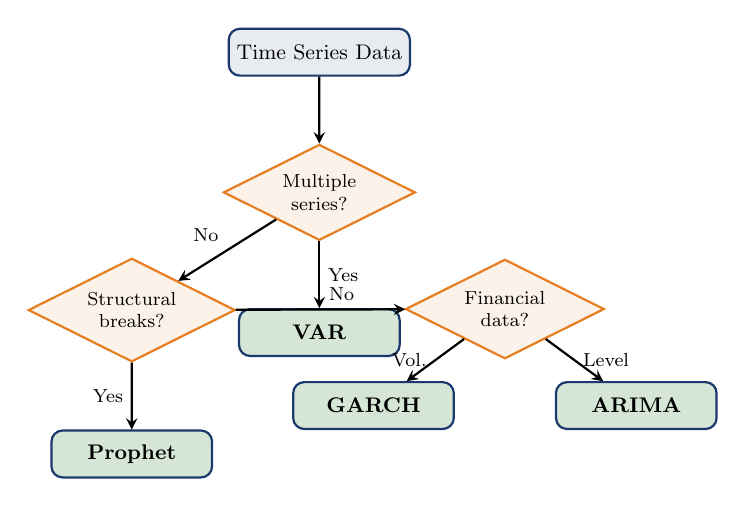
\begin{tikzpicture}[scale=0.85, transform shape,
        node distance=1.0cm,
        box/.style={rectangle, draw=MainBlue, thick, fill=MainBlue!10, rounded corners, minimum width=2.4cm, minimum height=0.7cm, align=center, font=\small},
        decision/.style={diamond, draw=Orange, thick, fill=Orange!10, aspect=2, align=center, font=\footnotesize},
        arrow/.style={->, thick, >=stealth}
    ]
        \node[box] (start) {Time Series Data};
        \node[decision, below=of start] (q1) {Multiple\\series?};
        \node[decision, below left=1.0cm and 1.3cm of q1] (q2) {Structural\\breaks?};
        \node[decision, below right=1.0cm and 1.3cm of q1] (q3) {Financial\\data?};
        \node[box, fill=Forest!20, below=of q1] (var) {\textbf{VAR}};
        \node[box, fill=Forest!20, below=of q2] (prophet) {\textbf{Prophet}};
        \node[box, fill=Forest!20, below left=0.7cm and 0cm of q3] (garch) {\textbf{GARCH}};
        \node[box, fill=Forest!20, below right=0.7cm and 0cm of q3] (arima) {\textbf{ARIMA}};
        \draw[arrow] (start) -- (q1);
        \draw[arrow] (q1) -- node[right] {\footnotesize Yes} (var);
        \draw[arrow] (q1) -- node[above left] {\footnotesize No} (q2);
        \draw[arrow] (q2) -- node[left] {\footnotesize Yes} (prophet);
        \draw[arrow] (q2) -- node[above right] {\footnotesize No} (q3);
        \draw[arrow] (q3) -- node[left] {\footnotesize Vol.} (garch);
        \draw[arrow] (q3) -- node[right] {\footnotesize Level} (arima);
    \end{tikzpicture}
    \end{center}
\end{frame}

\begin{frame}{Comprehensive Model Comparison}
    \begin{center}
    \footnotesize
    \begin{tabular}{lcccc}
        \toprule
        \textbf{Feature} & \textbf{GARCH} & \textbf{Fourier} & \textbf{Prophet} & \textbf{VAR} \\
        \midrule
        \textbf{Target} & Volatility & Level & Level & Multiple \\
        \textbf{Seasonality} & No & Yes (long) & Yes (multi) & No \\
        \textbf{Structural breaks} & No & No & Yes & No \\
        \textbf{Multiple series} & No & No & No & Yes \\
        \textbf{Interpretable} & Medium & High & High & High \\
        \textbf{Parameters} & Few & $2K$ & Auto & Many \\
        \textbf{Missing data} & No & No & Yes & No \\
        \midrule
        \textbf{Best for} & Finance & Cycles & Business & Macro \\
        \bottomrule
    \end{tabular}
    \end{center}

    \vspace{0.3cm}

    \begin{columns}[T]
        \column{0.5\textwidth}
        \begin{block}{Empirical Conclusions}
            \begin{itemize}\setlength{\itemsep}{0pt}
                \item \textbf{GARCH}: Student-t $>$ Normal ($\Delta$AIC = 509)
                \item \textbf{Fourier}: $K=3$ harmonics, validated on validation set
                \item \textbf{Prophet}: adapts to breaks via changepoints
                \item \textbf{VAR}: significant macro interactions (Granger)
            \end{itemize}
        \end{block}

        \column{0.5\textwidth}
        \begin{exampleblock}{Key Insight}
            \begin{itemize}\setlength{\itemsep}{0pt}
                \item RMSE cannot be compared across different datasets!
                \item Each model excels in its domain
                \item The art: matching model $\leftrightarrow$ data
            \end{itemize}
        \end{exampleblock}
    \end{columns}
\end{frame}

\begin{frame}{Best Practices for Applied Forecasting}
    \footnotesize
    \begin{columns}[T]
        \column{0.5\textwidth}
        \begin{block}{Methodology}
            \begin{enumerate}\setlength{\itemsep}{0pt}
                \item \textbf{Explore} data
                \item \textbf{Test} stationarity
                \item \textbf{Split} train/val/test
                \item \textbf{Compare} on validation
                \item \textbf{Report} test metrics
            \end{enumerate}
        \end{block}

        \begin{alertblock}{Common Mistakes}
            \begin{itemize}\setlength{\itemsep}{0pt}
                \item Peeking at test data
                \item Over-fitting
                \item Ignoring assumptions
            \end{itemize}
        \end{alertblock}

        \column{0.5\textwidth}
        \begin{exampleblock}{Practical Tips}
            \begin{itemize}\setlength{\itemsep}{0pt}
                \item Start simple (naive)
                \item Add complexity if needed
                \item Check residuals
                \item Report CIs
            \end{itemize}
        \end{exampleblock}

        \begin{block}{Remember}
            ``All models are wrong, but some are useful.'' --- Box
        \end{block}
    \end{columns}
\end{frame}

%=============================================================================
% CONCLUSION
%=============================================================================

\begin{frame}{Forecasting vs Causality vs Decision}
    \begin{center}
    \footnotesize
    \begin{tabular}{lll}
        \toprule
        \textbf{Objective} & \textbf{Model} & \textbf{Focus} \\
        \midrule
        Pure prediction & ARIMA / ML & Out-of-sample accuracy \\
        Financial risk & GARCH & Volatility, VaR \\
        Macro dynamics & VAR & Multivariate interactions \\
        Structural relations & SVAR / VECM & Causal identification \\
        Regimes & Markov Switching & Regime changes \\
        \bottomrule
    \end{tabular}
    \end{center}

    \vspace{0.3cm}

    \begin{alertblock}{Key Message}
        \begin{itemize}\setlength{\itemsep}{0pt}
            \item There is no universal model
            \item There is \textbf{fit between model and problem}
        \end{itemize}
    \end{alertblock}
\end{frame}

\begin{frame}{Key Takeaways}
    \begin{cminipage}{0.95\textwidth}
    \small
    \begin{enumerate}
        \item \textbf{Rigorous Methodology}
        \begin{itemize}
            \item Train/validation/test split prevents overfitting
            \item Test set must remain untouched until final evaluation
        \end{itemize}

        \vspace{0.2cm}

        \item \textbf{Match Model to Data}
        \begin{itemize}
            \item Financial volatility $\rightarrow$ GARCH
            \item Long seasonality $\rightarrow$ Fourier terms
            \item Structural breaks $\rightarrow$ Prophet
            \item Multiple series $\rightarrow$ VAR
        \end{itemize}

        \vspace{0.2cm}

        \item \textbf{Interpret Results Carefully}
        \begin{itemize}
            \item Granger causality $\neq$ true causality
            \item Out-of-sample performance matters most
            \item Simpler models often work better
        \end{itemize}
    \end{enumerate}
    \end{cminipage}
\end{frame}

%=============================================================================
\section{AI Use Case}
%=============================================================================

\begin{frame}{The Role of AI in Time Series Modeling}
    \begin{columns}[T]
        \column{0.5\textwidth}
        \begin{exampleblock}{AI can}
            \begin{itemize}\setlength{\itemsep}{0pt}
                \item Generate code for estimation and forecasting
                \item Select models (AutoML, grid search)
                \item Combine forecasts (ensemble)
                \item Detect anomalies and patterns
            \end{itemize}
        \end{exampleblock}

        \column{0.5\textwidth}
        \begin{alertblock}{But cannot}
            \begin{itemize}\setlength{\itemsep}{0pt}
                \item Replace statistical validation
                \item Automatically detect \textbf{data leakage}
                \item Guarantee correct economic interpretation
                \item Verify model assumptions
            \end{itemize}
        \end{alertblock}
    \end{columns}

    \vspace{0.3cm}

    \begin{block}{Principle}
        \begin{itemize}\setlength{\itemsep}{0pt}
            \item AI is a \textbf{tool}, not an authority
            \item Statistical validation remains the researcher's responsibility
        \end{itemize}
    \end{block}
\end{frame}

\begin{frame}{AI Exercise: Critical Thinking}
    \begin{cminipage}{0.95\textwidth}
    \vspace{-3mm}
    \begin{block}{\footnotesize Prompt to test in ChatGPT / Claude / Copilot}
        {\footnotesize
        ``Download monthly US Retail Sales from FRED (series RSXFS) for 2010-01 to 2024-12 (180 observations). Perform a complete time series analysis: decomposition, stationarity tests, model selection (compare ETS, SARIMA, and Prophet), 12-month forecast, and evaluation using RMSE/MAE/MASE on a 70/15/15 temporal split. Give me publication-quality Python code.''
        }
    \end{block}
    \vspace{-2mm}
    {\footnotesize
    \textbf{Exercise}:
    \begin{enumerate}\setlength{\itemsep}{0pt}
        \item Run the prompt in an LLM of your choice and critically analyze the response.
        \item Does it follow the correct workflow? (plot $\to$ decompose $\to$ test $\to$ model $\to$ diagnose $\to$ forecast)
        \item Does it compare multiple models (ETS, ARIMA, SARIMA) with proper benchmarks?
        \item Is the train/test split done properly? Is there any data leakage?
        \item Does it discuss limitations and assumptions of the chosen model?
    \end{enumerate}
    }
    \vspace{-2mm}
    \begin{alertblock}{}
        {\footnotesize \textbf{Warning}: AI-generated code may run without errors and look professional. \textit{That does not mean it is correct.}}
    \end{alertblock}
    \end{cminipage}
\end{frame}

%=============================================================================
% QUIZ
%=============================================================================
\section{Quiz}

\begin{frame}{Question 1}
    \begin{cminipage}{0.95\textwidth}
    \begin{alertblock}{Question}
        \begin{itemize}\setlength{\itemsep}{0pt}
            \item Which model would you choose to forecast the volatility of financial returns?
        \end{itemize}
    \end{alertblock}

    \vspace{0.3cm}

    \begin{block}{Answer Choices}

        \textcolor{MainBlue}{\textbf{(A)}} ARIMA --- captures trends and autocorrelations\\[3pt]

        \textcolor{MainBlue}{\textbf{(B)}} GARCH --- models conditional variance\\[3pt]

        \textcolor{MainBlue}{\textbf{(C)}} Prophet --- detects changepoints and seasonality\\[3pt]

        \textcolor{MainBlue}{\textbf{(D)}} VAR --- multivariate model for interdependencies

    \end{block}
    \end{cminipage}
\end{frame}

\begin{frame}{Question 1: Answer}
    \begin{cminipage}{0.95\textwidth}
    \vspace{-0.2cm}
    \begin{center}
        \includegraphics[width=0.98\textwidth, height=0.58\textheight, keepaspectratio]{ch10_quiz1_model_selection.pdf}
    \end{center}
    \vspace{-3mm}
    {\small
    \begin{exampleblock}{Answer: (B)}
    \begin{itemize}\setlength{\itemsep}{0pt}
        \item GARCH captures volatility clustering and time-varying risk. ARIMA models the level, Prophet handles seasonality, VAR captures cross-series dynamics --- none model variance directly.
    \end{itemize}
    \end{exampleblock}
    }
    \hfill\quantlet{TSA\_ch10\_quiz1\_model\_selection}{https://github.com/QuantLet/TSA/tree/main/TSA_ch10/TSA_ch10_quiz1_model_selection}
    \end{cminipage}
\end{frame}

\begin{frame}{Question 2}
    \begin{cminipage}{0.95\textwidth}
    \begin{alertblock}{Question}
        \begin{itemize}\setlength{\itemsep}{0pt}
            \item A SARIMA model achieves RMSE = 0.05 on training but RMSE = 2.30 on test. What does this indicate?
        \end{itemize}
    \end{alertblock}

    \vspace{0.3cm}

    \begin{block}{Answer Choices}

        \textcolor{MainBlue}{\textbf{(A)}} The model is excellent --- low training error confirms quality\\[3pt]

        \textcolor{MainBlue}{\textbf{(B)}} The model suffers from overfitting --- it memorizes noise\\[3pt]

        \textcolor{MainBlue}{\textbf{(C)}} The test set is faulty and should be replaced\\[3pt]

        \textcolor{MainBlue}{\textbf{(D)}} The difference is normal --- all models have higher test error

    \end{block}
    \end{cminipage}
\end{frame}

\begin{frame}{Question 2: Answer}
    \begin{cminipage}{0.95\textwidth}
    \vspace{-0.2cm}
    \begin{center}
        \includegraphics[width=0.98\textwidth, height=0.58\textheight, keepaspectratio]{ch10_quiz2_overfitting.pdf}
    \end{center}
    \vspace{-3mm}
    {\small
    \begin{exampleblock}{Answer: (B)}
    \begin{itemize}\setlength{\itemsep}{0pt}
        \item A 46$\times$ ratio between test and training RMSE signals severe overfitting. The model fits noise in the training data and fails to generalize. Solution: simpler model, proper validation.
    \end{itemize}
    \end{exampleblock}
    }
    \hfill\quantlet{TSA\_ch10\_quiz2\_overfitting}{https://github.com/QuantLet/TSA/tree/main/TSA_ch10/TSA_ch10_quiz2_overfitting}
    \end{cminipage}
\end{frame}

\begin{frame}{Question 3}
    \begin{cminipage}{0.95\textwidth}
    \begin{alertblock}{Question}
        \begin{itemize}\setlength{\itemsep}{0pt}
            \item Why is it important to separate data into train/validation/test sets?
        \end{itemize}
    \end{alertblock}

    \vspace{0.3cm}

    \begin{block}{Answer Choices}

        \textcolor{MainBlue}{\textbf{(A)}} To have more training data\\[3pt]

        \textcolor{MainBlue}{\textbf{(B)}} To prevent overfitting and evaluate correctly\\[3pt]

        \textcolor{MainBlue}{\textbf{(C)}} It is just a convention with no real importance\\[3pt]

        \textcolor{MainBlue}{\textbf{(D)}} To reduce computation time

    \end{block}
    \end{cminipage}
\end{frame}

\begin{frame}{Question 3: Answer}
    \begin{cminipage}{0.95\textwidth}
    \vspace{-0.2cm}
    \begin{center}
        \includegraphics[width=0.98\textwidth, height=0.58\textheight, keepaspectratio]{ch10_quiz3_train_val_test.pdf}
    \end{center}
    \vspace{-3mm}
    {\small
    \begin{exampleblock}{Answer: (B)}
    \begin{itemize}\setlength{\itemsep}{0pt}
        \item Train: estimate parameters. Validation: select model/hyperparameters. Test: final unbiased evaluation. Mixing these roles leads to optimistic performance estimates.
    \end{itemize}
    \end{exampleblock}
    }
    \hfill\quantlet{TSA\_ch10\_quiz3\_train\_val\_test}{https://github.com/QuantLet/TSA/tree/main/TSA_ch10/TSA_ch10_quiz3_train_val_test}
    \end{cminipage}
\end{frame}

\begin{frame}{Question 4}
    \begin{cminipage}{0.95\textwidth}
    \begin{alertblock}{Question}
        \begin{itemize}\setlength{\itemsep}{0pt}
            \item Is Granger causality equivalent to true (structural) causality?
        \end{itemize}
    \end{alertblock}

    \vspace{0.3cm}

    \begin{block}{Answer Choices}

        \textcolor{MainBlue}{\textbf{(A)}} Yes --- if $X$ predicts $Y$, then $X$ causes $Y$\\[3pt]

        \textcolor{MainBlue}{\textbf{(B)}} No --- it only tests predictive content, not causation\\[3pt]

        \textcolor{MainBlue}{\textbf{(C)}} It depends on the number of lags selected\\[3pt]

        \textcolor{MainBlue}{\textbf{(D)}} Yes, if the p-value is below 0.05

    \end{block}
    \end{cminipage}
\end{frame}

\begin{frame}{Question 4: Answer}
    \begin{cminipage}{0.95\textwidth}
    \vspace{-0.2cm}
    \begin{center}
        \includegraphics[width=0.98\textwidth, height=0.58\textheight, keepaspectratio]{ch10_quiz4_granger_causality.pdf}
    \end{center}
    \vspace{-3mm}
    {\small
    \begin{exampleblock}{Answer: (B)}
    \begin{itemize}\setlength{\itemsep}{0pt}
        \item Granger causality tests whether past $X$ improves forecasts of $Y$. Spurious correlations (e.g., ice cream sales and drownings) can pass the test due to common causes.
    \end{itemize}
    \end{exampleblock}
    }
    \hfill\quantlet{TSA\_ch10\_quiz4\_granger\_causality}{https://github.com/QuantLet/TSA/tree/main/TSA_ch10/TSA_ch10_quiz4_granger_causality}
    \end{cminipage}
\end{frame}

\begin{frame}{Question 5}
    \begin{cminipage}{0.95\textwidth}
    \begin{alertblock}{Question}
        \begin{itemize}\setlength{\itemsep}{0pt}
            \item What model do you use for a series with long seasonality (e.g., $s = 365$ days)?
        \end{itemize}
    \end{alertblock}

    \vspace{0.3cm}

    \begin{block}{Answer Choices}

        \textcolor{MainBlue}{\textbf{(A)}} SARIMA$(p,d,q)(P,D,Q)_{365}$\\[3pt]

        \textcolor{MainBlue}{\textbf{(B)}} GARCH --- models variation\\[3pt]

        \textcolor{MainBlue}{\textbf{(C)}} ARIMA + Fourier terms or Prophet/TBATS\\[3pt]

        \textcolor{MainBlue}{\textbf{(D)}} VAR with 365 lags

    \end{block}
    \end{cminipage}
\end{frame}

\begin{frame}{Question 5: Answer}
    \begin{cminipage}{0.95\textwidth}
    \vspace{-0.2cm}
    \begin{center}
        \includegraphics[width=0.98\textwidth, height=0.58\textheight, keepaspectratio]{ch10_quiz5_long_seasonality.pdf}
    \end{center}
    \vspace{-3mm}
    {\small
    \begin{exampleblock}{Answer: (C)}
    \begin{itemize}\setlength{\itemsep}{0pt}
        \item SARIMA$_{365}$ requires lag polynomials of order 365 --- computationally infeasible. Fourier terms with $K=3$ use only 6 parameters ($\sin$/$\cos$). Prophet and TBATS handle multiple seasonalities automatically.
    \end{itemize}
    \end{exampleblock}
    }
    \hfill\quantlet{TSA\_ch10\_quiz5\_long\_seasonality}{https://github.com/QuantLet/TSA/tree/main/TSA_ch10/TSA_ch10_quiz5_long_seasonality}
    \end{cminipage}
\end{frame}

\begin{frame}{Bibliography I}
    \begin{block}{Fundamental Textbooks (common references across all chapters)}
        {\small
        \begin{itemize}
            \item Hamilton, J.D. (1994). \textit{Time Series Analysis}, Princeton University Press.
            \item Hyndman, R.J., \& Athanasopoulos, G. (2021). \textit{Forecasting: Principles and Practice}, 3rd ed., OTexts.
            \item Shumway, R.H., \& Stoffer, D.S. (2017). \textit{Time Series Analysis and Its Applications}, 4th ed., Springer.
        \end{itemize}
        }
    \end{block}

    \begin{exampleblock}{Domain-Specific References}
        {\small
        \begin{itemize}
            \item Tsay, R.S. (2010). \textit{Analysis of Financial Time Series}, 3rd ed., Wiley. (GARCH, VAR)
            \item Lütkepohl, H. (2005). \textit{New Introduction to Multiple Time Series Analysis}, Springer. (VAR, VECM)
            \item Francq, C., \& Zakoïan, J.-M. (2019). \textit{GARCH Models}, 2nd ed., Wiley. (Volatility)
        \end{itemize}
        }
    \end{exampleblock}
\end{frame}

\begin{frame}{Bibliography II}
    \begin{block}{Modern Approaches and Forecasting Competitions}
        {\small
        \begin{itemize}
            \item Petropoulos, F., et al. (2022). Forecasting: Theory and Practice, \textit{International Journal of Forecasting}, 38(3), 845--1054.
            \item Makridakis, S., Spiliotis, E., \& Assimakopoulos, V. (2020). The M4 Competition, \textit{International Journal of Forecasting}, 36(1), 54--74.
            \item Taylor, S.J., \& Letham, B. (2018). Forecasting at Scale, \textit{The American Statistician}, 72(1), 37--45.
        \end{itemize}
        }
    \end{block}
\end{frame}

%=============================================================================
% SUMMARY
%=============================================================================
\section{Summary}

\begin{frame}{Course Summary}
\begin{block}{What We Learned}
\begin{itemize}
    \item Model selection depends on data characteristics: stationarity, seasonality, volatility
    \item The Box-Jenkins methodology provides a systematic framework for time series modeling
    \item Proper evaluation requires out-of-sample testing and time series cross-validation
\end{itemize}
\end{block}

\begin{alertblock}{Important}
No single model wins everywhere. Match the model to the data: ARIMA for trends, SARIMA for seasonality, GARCH for volatility, VAR/VECM for multivariate dynamics, Prophet/TBATS for complex patterns. Always validate out-of-sample!
\end{alertblock}
\end{frame}

%=============================================================================
% REFERENCES
%=============================================================================
\begin{frame}{References}
    \footnotesize
    \begin{thebibliography}{99}
        \bibitem{box2015} Box, G.E.P., Jenkins, G.M., Reinsel, G.C., \& Ljung, G.M. (2015). \textit{Time Series Analysis: Forecasting and Control}. 5th ed., Wiley.

        \bibitem{hamilton1994} Hamilton, J.D. (1994). \textit{Time Series Analysis}. Princeton University Press.

        \bibitem{tsay2010} Tsay, R.S. (2010). \textit{Analysis of Financial Time Series}. 3rd ed., Wiley.

        \bibitem{hyndman2021} Hyndman, R.J., \& Athanasopoulos, G. (2021). \textit{Forecasting: Principles and Practice}. 3rd ed., OTexts.

        \bibitem{taylor2018} Taylor, S.J., \& Letham, B. (2018). Forecasting at Scale. \textit{The American Statistician}, 72(1), 37-45.

        \bibitem{bollerslev1986} Bollerslev, T. (1986). Generalized Autoregressive Conditional Heteroskedasticity. \textit{Journal of Econometrics}, 31(3), 307-327.

        \bibitem{sims1980} Sims, C.A. (1980). Macroeconomics and Reality. \textit{Econometrica}, 48(1), 1-48.
    \end{thebibliography}
\end{frame}

\begin{frame}{}
    \centering
    \Huge\textcolor{MainBlue}{Thank You!}

    \vspace{1cm}

    \Large Questions?

    \vspace{0.8cm}

    \normalsize

    Course materials available at: \url{https://danpele.github.io/Time-Series-Analysis/}

    \vspace{0.2cm}

    \href{https://quantlet.com}{\raisebox{-0.15em}{\includegraphics[height=0.8em]{ql_logo.png}} Quantlet} \hspace{0.5cm}
    \href{https://quantinar.com}{\raisebox{-0.15em}{\includegraphics[height=0.8em]{qr_logo.png}} Quantinar}
\end{frame}

\end{document}
